%CLASSE DOCUMENTO - LINGUA E DIMENSIONE FONT
\documentclass[corpo=10pt,numerazioneromana]{toptesi}

%%%%%%%%%%%%%%%%%%%%%%%%%%%%%%%%%%%%%%%%%%%%%%%%%%%%%%%%%%%%%%%

% INCLUSIONE PACCHETTI
\usepackage[classica]{topfront}
\usepackage[utf8]{inputenc} %utf8
\usepackage[italian]{babel}
\usepackage[T1]{fontenc}
\usepackage{blindtext}
\usepackage{graphicx,wrapfig}
\usepackage{booktabs}
\usepackage{lmodern}
\usepackage{varioref}
\usepackage{url}
\usepackage{array}
\usepackage{paralist}{\obeyspaces\global\let =\space}
\usepackage{verbatim}
\usepackage{subfig}
\usepackage{tabularx}
\usepackage{amsmath}
\usepackage{amsfonts}
\usepackage{float}
\usepackage{amssymb}
\usepackage{multicol}
\usepackage{multirow}
\usepackage{listings}
\usepackage[pass]{geometry}
\usepackage[figuresright]{rotating}
\usepackage{algorithm}
\usepackage{algorithmic}
\usepackage{amsmath}
\usepackage[babel]{csquotes}
\usepackage{hyperref}
\usepackage{fancyhdr}
\usepackage{indentfirst}
\usepackage[font=small,labelfont=bf]{caption}

%% this for both bibliography and sitografia
% \usepackage[round]{natbib}
% \usepackage{multibib}
% \newcites{Math}{Sitografia}

%% only bibliography
%%%%5 style=numeric-comp
\usepackage[backend=biber, bibencoding=utf8, style=numeric-comp, sorting=none]{biblatex}
% \usepackage[backend=biber, bibencoding=ascii]{biblatex}

%%%%%%%%%%%%%%%%%%%%%%%%%%%%%%%%%%%%%%%%%%%%%%%%%%%%%%%%%%%%%%%

%INTERLINEA
\interlinea{1.5}

%%%%%%%%%%%%%%%%%%%%%%%%%%%%%%%%%%%%%%%%%%%%%%%%%%%%%%%%%%%%%%%

% CONFIGURAZIONE LINK E RIFERIMENTI
\hypersetup{%
    pdfpagemode={UseOutlines},
    bookmarksopen,
    pdfstartview={FitH},
    colorlinks,
    linkcolor={black}, %COLORE DEI RIFERIMENTI AL TESTO
    citecolor={blue}, %COLORE DEI RIFERIMENTI ALLE CITAZIONI
    urlcolor={blue} %COLORI DEGLI URL
}

%%%%%%%%%%%%%%%%%%%%%%%%%%%%%%%%%%%%%%%%%%%%%%%%%%%%%%%%%%%%%%%

% CONFIGURAZIONE LISTATI/CODICE - CANCELLARE SE NON NECESSARIO
% PYTHON - BIANCO E NERO
\lstset{%
	captionpos=b,
	language=Python,
	basicstyle =\small\ttfamily,
	keywordstyle=\color{black}\bfseries,
	breaklines=true,
	breakatwhitespace=true,
	frame=lines,
	numbers=left,
	numberstyle=\footnotesize,
}

%%%%%%%%%%%%%%%%%%%%%%%%%%%%%%%%%%%%%%%%%%%%%%%%%%%%%%%%%%%%%%%

% FRENCHSPACING VA _SEMPRE_ ABILITATO PER DOCUMENTI IN ITALIANO
\frenchspacing

%%%%%%%%%%%%%%%%%%%%%%%%%%%%%%%%%%%%%%%%%%%%%%%%%%%%%%%%%%%%%%%

%DEFINIZIONE SEZIONI IN NUMERAZIONE ROMANA
%ELENCO DEI LISTATI/CODICI
\newcommand\myfontsize{\fontsize{11pt}{13pt}\selectfont}

\makeatletter
\newcommand\listofcodes{%
 \iffrontmatter\else\frontmattertrue\fi
 \if@openright\cleardoublepage\else\clearpage\fi
 % change the meaning of \chapter in a group
 \begingroup\def\chapter##1{\@schapter}
 \phantomsection % for the hyperlink
 \addcontentsline{toc}{chapter}{Elenco dei Codici}
 \lstlistoflistings
 \endgroup
} 
\makeatother

\addto\captionsitalian{%
  \renewcommand{\lstlistlistingname}{Elenco dei Codici}%
  \renewcommand{\lstlistingname}{Codice}%
  \renewcommand{\listfigurename}{Elenco delle Figure}%
}

%%%%%%%%%%%%%%%%%%%%%%%%%%%%%%%%%%%%%%%%%%%%%%%%%%%%%%%%%%%%%%%

%%%%%%%%%%%%%%%%%%%%%%%%%%%%%%%%%%%%%%%%%%%%%%%%%%%%%%%%%%%%%%%

%%% LISTA DEI CAPITOLI DA INCLUDERE - PERSONALIZZARE
\includeonly{%
fronte,%
introduzione,%
chap_1,%
chap_2,%
chap_3,%
conclusioni,%
app_a,%
ringraziamenti,%
}

%%%% FILE DI BIBLIOGRAFIA
\addbibresource{bibliography.bib}
\AtBeginBibliography{\small}


%%%%%%%%%%%%%%%%%%%%%%%%%%%%%%%%%%%%%%%%%%%%%%%%%%%%%%%%%%%%%%%



% INIZIO DOCUMENTO
\begin{document}


%%%%%%%%%%%%%%%%%%%%%%%%%%%%%%%%%%%%%%%%%%%%%%%%%%%%%%%%%%%%%%%
%%% DEFINE CODE STYLES %%%
\definecolor{javared}{rgb}{0.6,0,0} % for strings
\definecolor{javagreen}{rgb}{0.25,0.5,0.35} % comments
\definecolor{javapurple}{rgb}{0.5,0,0.35} % keywords
\definecolor{javadocblue}{rgb}{0.25,0.35,0.75} % javadoc

\lstset{language=Java,
otherkeywords={
        String, boolean, int, double, float, @NotNull, @Size, @RequestHeader
        },
basicstyle=\ttfamily,
keywordstyle=\color{javapurple}\bfseries,
stringstyle=\color{javared},
commentstyle=\color{javagreen},
morecomment=[s][\color{javadocblue}]{/**}{*/},
numbers=none,
numberstyle=\color{black},
stepnumber=2,
numbersep=10pt,
tabsize=4,
showspaces=false,
frame=leftline,
showstringspaces=false}

\lstset{language=HTML,
otherkeywords={
        % HTML tags
        <html>, <head>, <title>, </title>, <meta, />, </head>, <body>, <app-form, <app-outcome, <app-offline, /app-form>, /app-outcome>, /app-offline>,
        <canvas, \/canvas>, <script>, </script>, </body>, </html>, <!, html>, <style>, </style>, ><
        },
ndkeywords={[ngClass], (notify)},
basicstyle=\fontsize{10}{12}\selectfont\ttfamily,
keywordstyle=\color{blue}\bfseries,
ndkeywordstyle=\color{javapurple}\bfseries,
stringstyle=\color{javagreen},
commentstyle=\color{javared},
morecomment=[s][\color{javadocblue}]{<!--}{-->},
numbers=none,
numberstyle=\color{black},
stepnumber=2,
numbersep=10pt,
tabsize=4,
showspaces=false,
frame=leftline,
showstringspaces=false}

%%%%%%%%%%%%%%%%%%%%%%%%%%%%%%%%%%%%%%%%%%%%%%%%%%%%%%%%%%%%%%%


\frontmatter
%%%%%%%%%%%%%%%%%%%%%%%%%%%%%%%%%%%%%%%%%%%%%%%%%%%%%%%%%%%%%%%


%%% REFERENZE
% This is a reference to a chapter \ref{chap:chap_2}. This is a reference to a figure \ref{fig:doge}. This is a reference to some code \ref{lst:hello}. This is a citation \cite{famous:paper}.




% CITAZIONE - PERSONALIZZARE
% VSPACE - PROPORZIONE USATA PER CENTRATURA VERTICALE DEL TESTO
% FLUSHRIGHT - ALLINEAMENTO ORIZZONTALE A DESTRA
% \vspace*{\stretch{1}}
% \begin{flushright}
% \noindent
% \textit{A Tobia e Bianca}

% \end{flushright}
% \vspace*{\stretch{6}}
% \cleardoublepage



%%%%%%%%%%%%%%%%%%%%%%%%%%%%%%%%%%%%%%%%%%%%%%%%%%%%%%%%%%%%%%%
%Intestazione
\thispagestyle{empty}

\begin{figure}[H]
  \centering
  
\includegraphics[width=0.2\textwidth]{img/logo_new_2022.png} 
  \label{fig:logo_new_2022.png}
\end{figure}

\begin{center}
    \textbf{\Large Università degli Studi di Torino} \\
    \textit{\Large Corso di Laurea in Informatica} \\
    \hfill \break
    \hfill \break
    \textbf{\huge Realizzazione di un servizio REST per la validazione dei codici bancari}\\
    {\Large Tesi di Laurea}
\end{center}
\vfill
\textbf{\Large Relatrice} \\
{\Large Liliana Ardissono}
\begin{flushright}
\hfill \break
\textbf{\Large Candidato:}\\
\textbf{\Large Luca Broggiato}\\
{\Large Matricola 916582}\\
\hfill \break
\hfill \break
\end{flushright}

\begin{center}
{\large Anno Accademico 2022/2023}
\end{center}

%INTERLINEA
\interlinea{2}

% ABSTRACT
\chapter*{Dichiarazione di Originalità}
\vspace{75pt}
{\large
\textit{Dichiaro di essere responsabile del contenuto dell’elaborato che presento al fine del conseguimento del titolo, di non avere plagiato in tutto o in parte il lavoro prodotto da altri e di aver citato le fonti originali in modo congruente alle normative vigenti in materia di plagio e di diritto d’autore. Sono inoltre consapevole che nel caso la mia dichiarazione risultasse mendace, potrei incorrere nelle sanzioni previste dalla legge e la mia ammissione alla prova finale potrebbe essere negata.}
}

\newpage
\chapter*{Abstract}
\vspace{75pt}
{\large
Con l'espansione continua dei servizi offerti dai gruppi bancari, l'importanza di avere un servizio di validazione degli ID degli account utente semplice, intuitivo e affidabile è più rilevante che mai. Questa tesi si propone di sviluppare tale servizio utilizzando i più recenti framework e tecnologie disponibili, mostrando anche la realizzazione una pagina web front-end che funge da punto di accesso per l'inserimento dei dati utente e da interfaccia visiva per l'output dell’elaborazione back-end. L'obiettivo principale di questa ricerca è stato fornire una soluzione efficace che soddisfi le esigenze attuali e future nel campo della validazione degli ID dei conti bancari, migliorando l'esperienza complessiva degli utenti.
}
% Sommario.

%INTERLINEA
\interlinea{1.5}

%%%%%%%%%%%%%%%%%%%%%%%%%%%%%%%%%%%%%%%%%%%%%%%%%%%%%%%%%%%%%%%
% INDICI - ELIMINARE GLI INDICI NON NECESSARI

% INDICE GENERALE
{\myfontsize
\tableofcontents
}

% INDICE DELLE FIGURE
%\listoffigures

%INDICE DELLE TABELLE
%\listoftables

% INDICE DEI CODICI
% \listofcodes
% \include{strumenti-ottici.py}
%%%%%%%%%%%%%%%%%%%%%%%%%%%%%%%%%%%%%%%%%%%%%%%%%%%%%%%%%%%%%%%

% INCLUSIONE FILE CAPITOLI - PERSONALIZZARE - TENERE COERENTE CON LISTA IN ALTO
\mainmatter
\chapter{Introduzione}
\label{chap:Introduzione}



La presente tesi descrive l'attività svolta durante il periodo di stage curricolare presso l'azienda multinazionale Alten, con sede a Torino. L'obiettivo centrale di questo studio è stato l'elaborazione di una soluzione dedicata alla verifica dei codici IBAN per un rinomato gruppo bancario di rilevanza europea. In tal senso, è stato ideato e sviluppato un applicativo volto a consentire all'utente di inserire il proprio codice IBAN per ottenere immediatamente una conferma circa la sua validità. Questo servizio è stato progettato con l'intento di costituire una risorsa di fondamentale importanza sia per la clientela retail, comprendente clienti individuali e persone fisiche, sia per il personale interno dell'istituto bancario.\\
Data la costante crescita dell'utenza bancaria e l'espansione continua dei servizi offerti, il numero di clienti all'interno del gruppo bancario è in costante aumento, una tendenza che si prevede proseguirà anche nei prossimi anni. Pertanto, l'accesso a un servizio semplice, intuitivo e soprattutto affidabile per la verifica e la validazione degli ID bancari è diventato fondamentale per tutte le operazioni relative ai conti correnti. Questa soluzione garantisce sia agli utenti sia agli operatori la possibilità di operare in modo sicuro e tempestivo.\\
Un aspetto altrettanto cruciale del progetto è stato il tracciamento delle operazioni eseguite attraverso il servizio, in modo da poter registrare le richieste, lo stato dell’elaborazione e le risposte correlate a ogni interazione. Questo requisito ha comportato l'implementazione di un database che è stato concepito per operare “in-memory”, ossia per archiviare e gestire i dati direttamente nella memoria principale del sistema: il vantaggio quindi consiste nel fatto che i dati vengano mantenuti nella RAM del computer, garantendo un accesso significativamente più rapido rispetto ai tradizionali database su disco.\\
Inoltre, poiché l’applicativo è reso disponibile anche ai clienti del gruppo bancario, la sua realizzazione ha richiesto l'utilizzo di linguaggi e tecnologie moderne e all'avanguardia. L'infrastruttura di back-end è stata sviluppata utilizzando il framework Spring Boot, il quale ha semplificato e al contempo ottimizzato l'implementazione del servizio REST. Infine, è stato utilizzato Spring Data JPA per la creazione e la gestione del database. Con “servizio REST” (dall’inglese REST service) si fa riferimento ad un tipo di architettura software utilizzata per la progettazione e l’esposizione di interfacce web che consentono alle applicazioni di comunicare e trasferire dati tramite il protocollo HTTP.\\
Tuttavia, il progetto non è limitato alla mera realizzazione del servizio back-end. È stato altresì necessario sviluppare un punto di accesso intuitivo e familiare sia per i clienti che per gli operatori: una pagina web. Con il vincolo di rispettare criteri di sicurezza, affidabilità, prestazioni e aspetto visivo, è stato adottato il framework open source Angular, che si presta alla creazione di applicazioni web dinamiche e complesse. La natura versatile di Angular lo rende particolarmente adatto allo sviluppo di applicazioni aziendali e di gestione dati, risultando un'opzione ideale per il servizio in questione.\\
Il secondo capitolo si focalizza sulle tecnologie utilizzate per la realizzazione dell’applicativo, ossia vengono presentati in maniera dettagliata i linguaggi di programmazione e i framework utilizzati sia per la realizzazione del comparto back-end, sia per quello front-end. Ci si sofferma, inoltre, sulle tecnologie più rilevanti nell'ambito dello sviluppo, senza analizzare le esatte implementazioni, che sono presenti nel capitolo successivo.\\
Il terzo capitolo è interamente dedicato al progetto. Infatti, offre un'analisi approfondita del contesto di lavoro, dell'attuazione pratica delle tecnologie precedentemente esaminate e dell'interazione interna, tra i membri del gruppo, ed esterna, tra le componenti front-end e back-end. Viene quindi illustrata la creazione del database e le procedure di persistenza dei dati, evidenziando le scelte relative a quali dati mantenere in memoria e le motivazioni sottostanti. Per finire, viene presentata la fase di test relativa al servizio back-end.\\
Il quarto capitolo costituisce la conclusione della tesi. Questa sezione riassume le parti principali esposte nell'elaborato e affronta questioni conclusive riguardanti il servizio realizzato, quali eventuali limitazioni dell’applicativo e possibili evoluzioni future attualmente non ancora implementate.




\chapter{Tecnologie Utilizzate}
\label{chap:Tecnologie Utilizzate}

Nel presente capitolo vengono presentate ed analizzate le tecnologie utilizzate per la realizzazione del progetto. I framework ed i linguaggi non sono trattati in relazione all’applicativo oggetto della tesi, bensì dal punto di vista meramente teorico e strutturale. 
L’ordine in cui le tecnologie sono presentate è stato pensato per mettere prima quelle riguardanti il lato back-end e successivamente quelle relative al front-end.

\section{Java}

Java è un linguaggio di programmazione ad alto livello, orientato agli oggetti e molto diffuso tra i programmatori. Viene ideato e distribuito dalla Sun Microsystems nei primi anni ‘90 con lo scopo di essere flessibile, affidabile e portatile, risultando subito uno strumento adatto alla programmazione per internet, che in quegli stessi anni inizia a diffondersi.
Tra la fine degli anni ‘90 ed i primi anni ‘00, Java acquista una notevole popolarità per via della sua versatilità, poiché permette di sviluppare applicazioni per il web, dispositivi mobili, computer, server e altro ancora. Inoltre, uno degli aspetti più importanti di Java, che ha aiutato a renderlo un linguaggio così diffuso, è la portabilità. Infatti, scrivendo un programma in Java, questo viene tradotto in un “formato speciale” (detto \textit{bytecode}) che non è direttamente eseguibile su una specifica piattaforma, ma che può essere eseguito dalla JVM (dall’inglese \textit{Java Virtual Machine}). Ciò consente ai programmi di funzionare su qualsiasi dispositivo che abbia una JVM adatta, a prescindere dal tipo di macchina o dal sistema operativo utilizzato. Nel 2010, Java viene acquisito da Oracle, a cui appartiene tuttora.\cite{JAVA_webopedia}\cite{JAVA_java}
Trattandosi di un linguaggio orientato agli oggetti, Java è progettato intorno al concetto di oggetti che interagiscono l’uno con l’altro, reciprocamente.

\subsection{Orientamento agli Oggetti}

L'orientamento agli oggetti è un paradigma di programmazione basato sulla rappresentazione di concetti del mondo reale come oggetti, che combinano stato (dati) e comportamento (funzioni) in un'unica entità. In un linguaggio di programmazione orientato agli oggetti, gli oggetti rappresentano le unità fondamentali di astrazione, intorno a cui è organizzato il programma.
In Java, gli oggetti rappresentano entità reali o concetti astratti all'interno del codice, che possono avere proprietà (variabili d'istanza) e comportamenti (metodi), potendo interagire tra loro attraverso lo scambio di messaggi.\cite{JAVA_unife}

\subsection{Vantaggi e Benefici}

I benefici dell’utilizzo di un linguaggio di programmazione orientato agli oggetti sono:
\begin{itemize}
    \item \textbf{Modularità e Riutilizzabilità}: gli oggetti consentono la suddivisione del codice in moduli autonomi e possono essere utilizzati in diverse parti del codice o in vari progetti, incrementando la manutenibilità e facilitando la creazione di sistemi complessi.\cite{JAVA_azionadigitale}
    \item \textbf{Incapsulamento}: le proprietà interne di un oggetto possono essere nascoste e rese accessibili solo attraverso metodi specifici, fornendo controllo sull’accesso ai dati.\cite{JAVA_educative}
    \item \textbf{Ereditarietà}: gli oggetti possono essere estesi attraverso l’ereditarietà, consentendo la creazione di nuove classi basate su classi esistenti e fornendo una gerarchia di classi per modellare i concetti.\cite{JAVA_educative}
    \item \textbf{Polimorfismo}: gli oggetti di classi diverse possono essere trattati in modo uniforme attraverso interfacce comuni, consentendo una gestione flessibile dei tipi di oggetti.\cite{JAVA_educative}
    \item \textbf{Astrazione}: l’astrazione consente di concentrarsi sui dettagli rilevanti e nascondere i dettagli di implementazione non necessari, semplificando la comprensione e l’utilizzo delle funzionalità.\cite{JAVA_educative}
    \item \textbf{Realismo}: l’orientamento agli oggetti consente di modellare e rappresentare concetti del mondo reale nel codice, rendendo più intuitiva la progettazione di soluzioni per problemi del mondo reale.
\end{itemize}


\subsection{Classi}

Le classi sono un concetto fondamentale nella programmazione orientata agli oggetti, dove formano la struttura che definisce un modello o il \textit{blueprint} per creare gli oggetti. Le classi descrivono sia le proprietà (dati) che i comportamenti (metodi) degli oggetti che vengono creati basandosi su di esse.
Nel contesto di un linguaggio come Java, le classi sono definite dai programmatori per rappresentare concetti specifici o entità del mondo reale. Di seguito, alcuni elementi chiave di una classe Java:
\begin{itemize}
    \item \textbf{campi} → rappresentano le proprietà o i dati associati ad un oggetto di quella classe;
    \item \textbf{metodi} → funzioni associate ad una classe, che definiscono il comportamento degli oggetti;
    \item \textbf{costruttori} → metodi speciali utilizzati per inizializzare gli oggetti di una classe, richiamati quando viene creato un nuovo oggetto della classe;
    \item \textbf{accessibilità} → le classi possono definire il livello di accesso ai loro campi e metodi (pubblico, privato, protetto). Questo determina quali parti del codice esterno possono interagire con la classe;
    \item \textbf{ereditarietà} → le classi possono ereditare proprietà e metodi da altre classi, consentendo la creazione di gerarchie di classi;
    \item \textbf{incapsulamento} → le classi consentono l’incapsulamento dei dati, quindi i campi interni possono essere protetti da accessi non autorizzati attraverso l’uso di livelli di accesso privati o protetti.
\end{itemize}
Le classi forniscono una forma di astrazione potente per organizzare il codice in modo modulare e rappresentare concetti del mondo reale in modo strutturato. L’uso appropriato delle classi favorisce la riutilizzabilità del codice, la chiarezza nella progettazione e l’organizzazione del software.\cite{JAVA_educative}\cite{JAVA_w3schools}

\subsection{Metodi}

Un programma Java è formato da più \textit{statement} (o istruzioni), che possono includere diversi tipi di dati. \`E possibile raggruppare questi elementi all'interno di uno o più metodi, richiamabili ed eseguibili varie volte.\\
I metodi sono blocchi di codice all’interno di una classe che eseguono una specifica operazione o azione. Nella programmazione orientata agli oggetti, i metodi rappresentano il comportamento degli oggetti creati da una classe e sono uno dei pilastri fondamentali, insieme ai campi (variabili d’istanza) e alla definizione di una classe.\cite{JAVA_educative}\cite{JAVA_w3schools2} Di seguito, alcune delle caratteristiche chiave dei metodi:
\begin{itemize}
    \item \textbf{comportamento} → i metodi definiscono cosa può fare un oggetto di una determinata classe;
    \item \textbf{riutilizzabilità} → i metodi sono definiti una volta e possono essere utilizzati su diversi oggetti creati dalla classe stessa o internamente ad altre classi. Ciò favorisce la modularità e la riduzione della duplicazione del codice;
    \item \textbf{parametri} → i metodi possono accettare parametri, che rappresentano il dominio della funzione. I parametri consentono di personalizzare l’azione del metodo in base alle necessità;
    \item \textbf{valore di ritorno} → i metodi possono restituire un valore, che rappresenta il codominio della funzione e corrisponde al risultato dell’esecuzione;
    \item \textbf{modificatori d’accesso} → i metodi possono avere specifici modificatori d’accesso (pubblico, privato o protetto) che ne definiscono la visibilità, per regolarne l’accesso;
    \item \textbf{overloading e overriding} → Java supporta il concetto di \textit{overloading} (sovraccarico), che consente di definire più versioni di un metodo cambiando solo i parametri. Inoltre, supporta l’\textit{overriding} (sovrascrittura), che permette ad una sottoclasse di fornire una nuova implementazione per un metodo ereditato dalla superclasse.
\end{itemize}

\subsection{Ereditarietà}

L’ereditarietà è un concetto fondamentale nella programmazione orientata agli oggetti, poiché consente di definire una nuova classe (detta sottoclasse o classe figlia) basata su una classe esistente (definita superclasse o classe genitore), ereditando le proprietà ed i comportamenti.\cite{JAVA_w3schools3} L’ereditarietà consente di creare una gerarchia di classi, semplificando la struttura del codice e favorendo la riutilizzabilità.\\
L’idea di base dell’ereditarietà è simile a quella di una gerarchia. Una sottoclasse eredita tutti i campi ed i metodi pubblici e protetti della superclasse. Ciò significa che la classe figlia può utilizzare e ampliare i membri della classe genitore senza doverli ripetere. Le classi possono essere organizzate in una struttura ad albero, con una singola classe radice (che in Java è Object) ed una o più sottoclassi. Questa gerarchia semplifica la rappresentazione dei concetti e la gestione delle funzionalità comuni.\cite{JAVA_educative}

\subsection{Sintassi e Statement}

L’istruzione (in inglese \textit{statement}) è la base della programmazione in Java. Si tratta di una singola operazione completa in grado di elaborare i dati dell’utente e può svolgere diversi compiti:
\begin{itemize}
    \item aggiungere oggetti;
    \item rimuovere oggetti;
    \item creare oggetti;
    \item invocare una funzione Java.\cite{JAVA_oracle}
\end{itemize}
Proprio come ogni linguaggio, anche lo \textit{statement} ha una sua sintassi, ovvero l’insieme di regole che definiscono come deve essere scritto. In Java, la sintassi è principalmente derivata da C e C++, ma a differenza di quest’ultimo, non esistono funzioni o variabili globali, bensì membri che sono considerati come tali. Ogni elemento del codice fa parte di una classe, e tutti i valori sono implicitamente oggetti. L’unica eccezione sono i tipi di dato primitivi, che non sono rappresentati da un’istanza di una classe per motivi di performance (nonostante possano essere convertiti automaticamente in oggetti e viceversa tramite un processo denominato \textit{autoboxing}\cite{JAVA_oracle2}). Alcune funzionalità, quali l’\textit{operator overloading} o i numeri interi senza segno, vengono omesse per semplificare il linguaggio ed evitare possibili errori.\\
Oltre a ciò, uno \textit{statement} fondamentale è rappresentato dalle strutture di controllo, ovvero meccanismi che permettono un controllo sul flusso di esecuzione del programma. Queste strutture consentono di eseguire azioni diverse in base a condizioni specifiche e di ripetere blocchi di codice o eseguire azioni alternative a seconda delle decisioni prese dal programma.

\subsection{Sistema di Tipi}

Java è un linguaggio \textit{type safe}, a tipizzazione statica, con un \textit{type system} nominativo e dotato di \textit{manifest typing}: per questi motivi, viene generalmente considerato un linguaggio a tipizzazione forte. Java distingue chiaramente i tipi primitivi, che definiscono valori atomici, dai tipi strutturati, che definiscono strutture composte. I tipi primitivi sono anche detti tipi atomici o tipi base e sono definiti nelle specifiche di linguaggio: per ognuno sono noti l’insieme esatto dei valori ammessi e gli operatori supportati.\\
I tipi strutturati sono anche tipi riferimento, cioè sono classi o interfacce che definiscono tipologie di oggetti. Tra queste, le classi degli array sono definite nelle specifiche di linguaggio, mentre tutti gli altri tipi strutturati sono \textit{user defined} (definiti dall’utente). I tipi definiti dall’utente legati al linguaggio sono riuniti nel 
\textit{package} \texttt{java.lang} e nei suoi sotto-\textit{package}. Il linguaggio stabilisce per alcuni di essi (quali \texttt{Object}, \texttt{String}, \texttt{Iterable} e altri) delle regole sintattiche o semantiche aggiuntive.\cite{JAVA_typesystem}

%% SPRING %%

\section{Spring}

Un framework è un insieme di librerie, strumenti e convenzioni che fornisce uno schema o una struttura per lo sviluppo di applicazioni. Il suo scopo è quello di semplificare il processo di sviluppo, consentendo ai programmatori di concentrarsi sulla logica specifica dell’applicazione piuttosto che sulle operazioni comuni e la gestione degli aspetti tecnici complessi.\cite{SPRING_amazon}\newline
Rilasciato nel Giugno del 2003 da Rod Johnson, Spring Framework (Spring) è un \textit{application framework open-source} di livello aziendale per lo sviluppo di applicazioni autonome basate su Java EE (Java Enterprise Edition)\cite{SPRING_techtarget}. È uno dei framework più popolari nel mondo dello sviluppo Java ed è noto per la sua flessibilità, facilità d’uso e capacità di affrontare una vasta gamma di problemi comuni nello sviluppo di applicazioni, aiutando lo sviluppatore nella creazione di software ad alte prestazioni con l’utilizzo semplici oggetti Java, chiamati in gergo tecnico POJO.\cite{SPRING_spring}

\subsection{Utilità}

Il motivo principale per cui nasce Spring è fornire una soluzione pratica alla complessità dei programmi Java. In questo senso, il framework offre un approccio sicuro, modulare e flessibile per costruire applicazioni, migliorando l’efficienza del codice e riducendo il tempo di sviluppo totale dell’applicazione. Inoltre, essendo efficiente nell’utilizzo delle risorse del sistema e fornendo supporto nella gestione dell’infrastruttura dell’applicazione, consente al programmatore di concentrarsi principalmente sulle funzionalità di business.
Di seguito, analizziamo nel dettaglio alcune delle peculiarità più significative del framework Spring.\cite{SPRING_spring}

\subsubsection{Componenti Principali di Spring}
\begin{itemize}
    \item \textbf{ApplicationContext} → è il cuore di Spring e rappresenta il \textit{container} che gestisce i \textit{bean}. Fornisce funzionalità avanzate quali la gestione dei cicli di vita dei \textit{bean}, la risoluzione delle dipendenze e altro ancora;\cite{SPRING_baeldung}
    \item \textbf{BeanFactory} → interfaccia sottostante dell’ApplicationContext, responsabile della creazione e gestione dei \textit{bean}. Inoltre, è il componente chiave per l’inversione di controllo;\cite{SPRING_spring2}
    \item \textbf{Bean} → oggetti definiti e gestiti dal container Spring;\cite{SPRING_baeldung}
    \item \textbf{Configurazioni} → le configurazioni supportate sono molte, tra cui \texttt{XML}, annotazioni (\texttt{@Component}, \texttt{@Autowired}, ecc…) e/o basate su Java, come \texttt{JavaConfig}. Le configurazioni definiscono come i \textit{bean} sono creati, regolati e collegati tra loro;\cite{SPRING_baeldung}
    \item \textbf{AOP (Aspect-Oriented Programming)} → le programmazione orientata agli aspetti consente di separare il codice che rappresenta le funzionalità trasversali (per esempio \textit{logging} e sicurezza) dalla logica di business principale;\cite{SPRING_spring3}
    \item \textbf{Aspetto Modulare} → Spring offre un ampio set di moduli che possono essere utilizzati in modo selettivo, in base alle esigenze dell’applicazione;\cite{SPRING_spring2}
\end{itemize}

\subsubsection{Inversione di Controllo (IoC - Inversion of Control)}

L'inversione di controllo (IoC), anche detta \textit{Inversion of Control}, permette una gestione più flessibile della creazione e del ciclo di vita degli oggetti (\textit{bean}) in un'applicazione. Questo approccio consente agli sviluppatori di concentrarsi sulla definizione del comportamento degli oggetti, mentre il \textit{container} Spring si occupa dell'istanziazione dei \textit{bean} e della risoluzione delle loro dipendenze. L'implementazione dell'IoC si basa sull'uso di configurazioni, come \textbf{XML}, annotazioni o codice Java.\cite{SPRING_italiancoders}\cite{SPRING_baeldung2}

\subsubsection{Iniezione delle Dipendenze (DI - Dependency Injection)}

L’iniezione delle dipendenze (DI) è un principio di progettazione software che consente di gestire le relazioni tra diversi componenti di un'applicazione in modo modulare e flessibile. In questo contesto, le dipendenze si riferiscono agli oggetti o alle risorse di cui un certo componente ha bisogno per svolgere le proprie operazioni.\\
Nell'ambito dello sviluppo di software, le applicazioni sono spesso composte da diverse parti o componenti che collaborano per raggiungere un obiettivo comune. Questi componenti possono avere dipendenze da altri componenti o risorse esterne, come librerie, database, servizi web e altro ancora.
La \textit{dependency injection} è un approccio che permette di gestire queste dipendenze esterne inversamente al metodo tradizionale. Invece di far sì che un componente crei le proprie dipendenze, il framework Spring si occupa di fornirle autonomamente,\cite{SPRING_italiancoders} di solito durante la fase di inizializzazione.
Gli sviluppatori definiscono di quali dipendenze necessita un componente tramite annotazioni o configurazioni, e Spring si preoccupa di fornirle quando l’elemento viene istanziato. Questo approccio comporta diversi vantaggi:
\begin{enumerate}
    \item \textbf{Disaccoppiamento}: i componenti diventano meno dipendenti l'uno dall'altro, rendendo il sistema più flessibile e facile da manutenere.
    \item \textbf{Riusabilità}: le dipendenze possono essere facilmente sostituite o aggiornate senza dover modificare il codice dei componenti che le utilizzano.
    \item \textbf{Testabilità}: è più semplice testare i singoli componenti in isolamento, poiché è possibile fornire dipendenze fittizie o simulate durante i test.
    \item \textbf{Leggibilità}: il codice diventa più chiaro e leggibile. Questo perché le dipendenze sono dichiarate in modo esplicito anziché "nascoste" all'interno dei componenti.
\end{enumerate}

\subsubsection{Flusso di Lavoro}

Spring fornisce un ambiente gestito (il \textit{container}) in cui gli sviluppatori definiscono le configurazioni e i componenti dell’applicazione.\cite{SPRING_tutorialspoint} Occupandosi di creazione, configurazione e gestione dei \textit{bean}, consente ai programmatori di concentrarsi sulla logica dell’applicazione, senza doversi preoccuparsi della gestione delle dipendenze e della creazione degli oggetti. Di seguito, il flusso di lavoro di Spring:
\begin{enumerate}
    \item l’applicazione definisce una (o più) configurazione Spring, la quale dichiara i \textit{bean}, le dipendenze e le regole di creazione;
    \item l’ApplicationContext (o la BeanFactory, a seconda della configurazione) carica e gestisce i \textit{bean} in base alle configurazioni fornite;
    \item l’applicazione interagisce con i \textit{bean} gestiti, che possono essere \textit{service}, \textit{controller}, componenti e altro ancora;
    \item le dipendenze tra i \textit{bean} sono gestite automaticamente da Spring tramite l’iniezione delle dipendenze.
\end{enumerate}
Quindi, la modularità, la flessibilità e le funzionalità di Spring lo rendono un framework estremamente popolare tra i programmatori Java per lo sviluppo di applicazioni di varie dimensioni e complessità.\cite{SPRING_javatechonline}

\subsection{Servizi WEB REST}

Un servizio WEB REST (\textit{Representational State Transfer}) è un tipo di servizio web basato su principi architetturali che utilizzano i protocolli standard del web, come HTTP, per consentire la comunicazione e lo scambio di dati tra \textit{client} e server in modo semplice, scalabile e senza stato\cite{SPRING_html}. I servizi web RESTful si basano sul concetto di risorse, che sono identificate da URL (\textit{Uniform Resource Locator}), e sfruttano le operazioni HTTP standard per l’accesso.\cite{SPRING_html2}
Le principali caratteristiche dei servizi web REST includono:
\begin{enumerate}
    \item \textbf{Utilizzo dei Metodi HTTP} → i metodi standard HTTP (quali \texttt{GET}, \texttt{PUT}, \texttt{POST}, \texttt{DELETE}) specificano l’operazione che deve essere eseguita su una risorsa, rendendo il servizio WEB RESTful coerente col protocollo;
    \item \textbf{Stateless} → ogni richiesta del \textit{client} deve contenere tutte le informazioni necessarie per comprenderla e gestirla. Il server non deve mantenere alcuno stato circa le richieste precedenti del \textit{client}, per semplificarne scalabilità e gestione;
    \item \textbf{Rappresentazione delle Risorse} → le risorse sono rappresentate usando formati standard come \texttt{JSON} o \texttt{XML}. I \textit{client} possono richiedere rappresentazioni specifiche delle risorse in base alle loro esigenze;
    \item \textbf{URI (Uniform Resource Identifier)} → ogni risorsa è identificata da un URI, che fornisce un modo standardizzato per accedervi tramite URL.
\end{enumerate}

\subsubsection{Integrazione Spring}

Per la realizzazione dei servizi WEB REST, i programmatori scelgono molto spesso di appoggiarsi a framework specifici. Uno dei framework più utilizzati in quest’ambito è proprio Spring, poiché semplifica notevolmente il processo di creazione del servizio. Al suo interno, la componente Spring MVC offre strumenti potenti e intuitivi per la definizione di API RESTful. Questo consente di gestire le richieste e le risposte in modo efficace, oltre ad automatizzare la conversione dei dati nei formati standard, come \texttt{JSON}. Un altro vantaggio chiave di Spring è la sua funzionalità di gestione delle dipendenze, caratteristica resa possibile dall’\textit{Inversion of Control} e dalla \textit{Dependency Injection}. Queste tecniche consentono di strutturare i servizi REST in modo che le dipendenze siano chiaramente definite e gestite in modo centralizzato, contribuendo a migliorare la manutenibilità e la testabilità del codice. Spring è altresì conosciuto per la sua capacità di integrazione semplificata con librerie e framework esterni. Questo significa che è possibile migliorare l’efficienza nello sviluppo utilizzando soluzioni standard per diverse situazioni, tra cui:
\begin{itemize}
    \item autenticazione;
    \item sicurezza;
    \item persistenza dei dati.
\end{itemize}
Un altro punto di forza di Spring è il supporto integrato per i formati standard. Questo semplifica la conversione dei dati tra oggetti Java e formati di rappresentazione comuni, agevolando l'interazione tra \textit{client} e server.\cite{SPRING_spring4}

\subsection{Java Spring Boot}

Java Spring Boot è uno strumento progettato per semplificare e velocizzare lo sviluppo di applicazioni web e microservizi utilizzando il framework Spring. Questo obiettivo è raggiunto attraverso tre funzionalità principali:
\begin{itemize}
    \item \textbf{Configurazione automatica}.
    \item \textbf{Approccio dichiarativo alla configurazione}.
    \item \textbf{Capacità di creare applicazioni autonome}.
\end{itemize}
L'integrazione di queste funzionalità fornisce uno strumento in grado di impostare applicazioni basate su Spring al costo di configurazioni ed installazioni minime.
Spring Boot consente di creare applicazioni rapidamente: analizzando il \textit{classpath} e i \textit{bean} configurati, fa delle ipotesi ragionevoli relative ai componenti mancanti e li aggiunge automaticamente, consentendo agli sviluppatori di concentrarsi sulle funzionalità di business anziché sull'infrastruttura.\cite{SPRINGBOOT_techwithmaddy}\cite{SPRINGBOOT_spring}
Tuttavia, è importante notare che nonostante la configurazione sia automatica, Spring Boot non interferisce con le personalizzazioni dell'utente. Ad esempio, se un utente ha definito una classe con impostazioni personalizzate per Thymeleaf, Spring Boot non aggiunge una seconda classe che sovrascriverebbe le impostazioni esistenti.
Inoltre, è importante sottolineare che Spring Boot non genera codice né modifica i file sorgente, bensì assembla i bean e le impostazioni e li applica al contesto dell'applicazione quando viene avviata.\cite{SPRINGBOOT_spring2}

\subsubsection{Funzionalità}

Il framework Spring Boot fornisce un modello di configurazione e una programmazione comprensibile per applicazioni \textit{enterprise} moderne basate su Java, che possono essere distribuite su qualsiasi piattaforma.\cite{SPRINGBOOT_ibm} Un elemento chiave di Spring è il suo supporto infrastrutturale a livello applicativo, che consente allo sviluppatore o al team di sviluppo di concentrarsi sulla logica di business dell'applicazione, senza vincoli specifici legati all'ambiente di distribuzione.\\
Inoltre, Spring Framework fornisce agli sviluppatori tutte le funzioni e gli strumenti necessari per creare applicazioni Java EE (Enterprise Edition) versatili, con un'ampia copertura di piattaforme ed eseguibili in diversi ambienti.\\
Spring Boot offre anche una funzionalità di \textit{Dependency Injection}, consentendo agli sviluppatori di creare applicazioni modulari formate da componenti debolmente accoppiati, ideali per servizi web ed applicazioni di rete distribuite.

\subsubsection{Integrazione}

Nonostante la sua potenza e completezza, Spring Framework richiede un notevole impegno in termini di tempo e competenze per essere configurato, impostato ed utilizzato all’interno delle applicazioni. Per rimediare a ciò si utilizza Spring Boot, che semplifica queste operazioni attraverso tre importanti funzionalità:
\begin{enumerate}
    \item \textbf{Configurazione Automatica} → Spring Boot offre una configurazione automatica iniziale che avvia le applicazioni fornendo alcune dipendenze preconfigurate, caratteristica che elimina la necessità della configurazione manuale. Inoltre, grazie a ciò il framework è in grado di impostare automaticamente sia il nucleo di Spring che le librerie di terze parti, rispettando le \textit{best practice} per prevenire errori.\cite{SPRINGBOOT_ibm}
    \item \textbf{Approccio Categorico} → Spring Boot adotta un approccio categorico per aggiungere e configurare le dipendenze iniziali, in base alle esigenze del progetto. Dopo una valutazione automatica, Spring seleziona i pacchetti da installare e i valori predefiniti da utilizzare. Questo evita all'utente la necessità di prendere queste decisioni e di configurare tutto manualmente.\cite{SPRINGBOOT_ibm}
    \item \textbf{Applicazioni Autonome} → Spring Boot agevola la creazione di applicazioni che possono essere eseguite autonomamente. Ad esempio, consente di sviluppare applicazioni che includono un server web integrato (come Tomcat o Netty) durante il processo di inizializzazione. Questo elimina la dipendenza da server web esterni e, di conseguenza, permette di avviare le applicazioni su qualsiasi piattaforma.\cite{SPRINGBOOT_ibm}
\end{enumerate}

\subsubsection{Architettura}

Spring Boot segue un'architettura formata da quattro livelli distinti, in cui ognuno comunica con quello precedente e successivo:
\begin{enumerate}
    \item Il \textbf{livello di presentazione} è il più alto dell'architettura. Le sue principali responsabilità includono l'autenticazione, la traduzione dei dati \texttt{JSON} in oggetti e la gestione delle richieste HTTP. In breve, questo livello gestisce l'interfaccia tra i \textit{client} e l'API REST, consentendo il flusso delle richieste verso il livello di business.\cite{SPRINGBOOT_techwithmaddy}\cite{SPRINGBOOT_javatpoint}
    \item Il \textbf{livello di business} è incaricato di gestire la logica di business, compresi processi di validazione e autorizzazione. Questo livello è costituito da classi di servizio e interagisce sia con il livello di presentazione che con il livello di persistenza. Il suo scopo è quello di implementare e gestire le regole e la logica dell'applicazione, determinando le azioni da compiere.\cite{SPRINGBOOT_techwithmaddy}\cite{SPRINGBOOT_javatpoint}
    \item Il \textbf{livello di persistenza} gestisce la logica di memorizzazione e traduce gli oggetti di business da e verso il database. Questo livello comunica direttamente sia il livello di business e con il livello di database, svolgendo un ruolo fondamentale nell'archiviazione dei dati e nella loro conversione in oggetti Java.\cite{SPRINGBOOT_techwithmaddy}\cite{SPRINGBOOT_javatpoint}
    \item Il \textbf{livello del database} è responsabile dell'esecuzione delle operazioni \texttt{CRUD} (crea, recupera, aggiorna, elimina). Rappresenta il database utilizzato per gestire i dati dell'applicazione, consentendo un’efficiente creazione e manipolazione delle informazioni.\cite{SPRINGBOOT_techwithmaddy}\cite{SPRINGBOOT_javatpoint}
\end{enumerate}


\subsection{Spring Boot e Spring Framework: confronto}

Sebbene Spring abbia reso più accessibile lo sviluppo delle applicazioni Java, può essere percepito come vasto e complesso da apprendere, a differenza di Spring Boot, che nasce proprio per risolvere questa situazione.\\
I principali vantaggi di Spring Boot rispetto a Spring Framework includono la facilità d'uso e la rapidità di sviluppo. In teoria, ciò potrebbe portare a una perdita di flessibilità rispetto all'uso diretto di Spring Framework. Tuttavia, nella pratica, a meno che non siano richieste configurazioni altamente personalizzate, l'adozione di Spring Boot rappresenta un valido compromesso.
Oltre a ciò, Spring Boot permette l’utilizzo del sistema di annotazioni di Spring, che può essere sfruttato per facilitare l'aggiunta di ulteriori dipendenze all'applicazione e l'accesso a tutte le funzionalità del Framework.\\
In ultima analisi, se il progetto è coperto anche da un solo Starter, Spring Boot rappresenta la scelta più indicata per agevolare lo sviluppo.\cite{SPRINGBOOT_techwithmaddy}\cite{SPRINGBOOT_ibm}

\subsection{Spring Data}
Spring Data fornisce un modello di programmazione per l'accesso ai dati basato su Spring, familiare e consistente, senza modificare il \textit{data store} in uso.
Semplifica l’utilizzo delle tecnologie per l'accesso ai dati, dei database (relazionali e non), dei framework \textit{map-reduce} e dei \textit{data services} basati su \textit{cloud}. Spring Data è quindi un progetto composto da sottoprogetti, specifici per il database in uso.\cite{SPRINGDATA_spring}

\subsubsection{JPA}

Java Persistence API è una specifica di Java EE che fornisce un framework per la gestione della persistenza dei dati in applicazioni Java. Dunque, JPA permette di memorizzare e recuperare dati da un database in modo efficace e standardizzato, utilizzando il linguaggio e gli oggetti Java anziché SQL.\cite{SPRINGDATA_ibm}\\
JPA offre un’astrazione sopra il database e fornisce un set di API che permettono agli sviluppatori di interagire con i dati in un modo orientato agli oggetti, senza dover scrivere direttamente \textit{query} SQL. Questo semplifica lo sviluppo di applicazioni e ne migliora la portabilità tra diversi database, poiché JPA si occupa delle specificità del database sottostante.
In JPA, le entità rappresentano le tabelle del database all'interno delle classi Java: ogni istanza di queste classi corrisponde a una riga nella tabella associata. L'interazione con le entità avviene principalmente attraverso l'EntityManager, un oggetto fondamentale che offre una serie di metodi per gestire le operazioni di salvataggio, aggiornamento, recupero ed eliminazione dei dati. Per definire come le classi delle entità sono mappate alle tabelle del database e per stabilire le relazioni tra di esse, si fa uso di annotazioni Java specifiche. In situazioni in cui è necessario effettuare query complesse, JPA sfrutta JPQL, un linguaggio di query orientato agli oggetti simile a SQL.\cite{SPRINGDATA_vincenzoracca}\\
Oltre a queste funzionalità, JPA offre un vantaggio notevole nell'automazione delle transazioni. Infatti, gestisce automaticamente le operazioni di transazione, assicurando che le sequenze di operazioni di lettura e scrittura si svolgano in modo coeso e che l'integrità dei dati sia preservata. Quindi, JPA semplifica in modo significativo la gestione dei dati persistenti attraverso l'uso di oggetti Java, consentendo agli sviluppatori di focalizzarsi sullo sviluppo logico dell'applicazione senza doversi preoccupare delle intricate complessità connesse al database.

\subsection{Spring Data JPA}

Spring Data JPA è parte del progetto Spring Data. Fornisce supporto avanzato per l'accesso ai dati e semplifica l'implementazione di \textit{repository} basati su JPA.\\
Infatti, implementare manualmente il livello di accesso ai dati per un'applicazione rappresenta un processo laborioso e complesso. Spesso, è necessario scrivere un gran quantitativo di codice di supporto, noto come \textit{boilerplate}, anche solo per eseguire operazioni di base, come \textit{query}, o per implementare funzionalità di paginazione e registrazione delle modifiche. In questo scenario trova spazio Spring Data JPA, che mira a semplificare l'implementazione del livello di accesso ai dati riducendo al minimo lo sforzo richiesto. L'obiettivo è ottimizzare l’implementazione, consentendo agli sviluppatori di focalizzarsi sulle esigenze specifiche del progetto. Invece di dover affrontare dettagli complessi e ripetitivi, i programmatori possono concentrarsi sulla creazione di interfacce per i \textit{repository}, che includono metodi per le operazioni di recupero e persistenza dei dati.\cite{SPRINGDATA_spring2}\\
Il punto di forza di Spring Data JPA è l’implementazione automatica delle interfacce definite, attuata da Spring “dietro le quinte”.\cite{SPRINGDATA_baeldung} Ciò permette ai programmatori di risparmiare tempo e risorse, non dovendosi occupare di scrivere manualmente il codice di ciascuna operazione.
In sostanza, Spring Data JPA agisce come un "ponte" tra gli sviluppatori e la complessità sottostante del livello di accesso ai dati, rendendo più efficiente lo sviluppo di applicazioni e consentendo ai programmatori di concentrarsi maggiormente sulla logica di business e sulle funzionalità dell'applicazione.

\subsubsection{Concetti Chiave}

Spring Data JPA semplifica l'interazione con il livello di persistenza dei dati grazie a funzionalità avanzate. Per fornire un supporto così importante, si basa su alcuni concetti chiave:
\begin{itemize}
    \item \textbf{Entity Classes}
    \begin{itemize}
        \item le classi entità sono normali classi Java annotate con metadati che definiscono la mappatura ai record del database, relazionando una classe o un attributo rispettivamente ad una tabella o a una colonna;
        \item le annotazioni JPA come \texttt{@Entity} o \texttt{@Id} specificano come le classi ed i campi debbano essere mappati ai dati del database.\cite{SPRINGDATA_baeldung2}
    \end{itemize}

    \item \textbf{Repository Interfaces}
    \begin{itemize}
        \item i programmatori definiscono interfacce di \textit{repository} estendendo \texttt{CrudRepository} o altre interfacce specifiche di Spring Data JPA;
        \item i \textit{repository} dichiarano metodi per l’accesso ai dati, come la ricerca, l’aggiornamento o la cancellazione, utilizzando le convenzioni di denominazione di Spring Data JPA.\cite{SPRINGDATA_baeldung3}
    \end{itemize}

    \item \textbf{Inversion of Control (IoC) \& Dependency Injection (DI)}
    \begin{itemize}
        \item Spring Data JPA sfrutta le caratteristiche di IoC e DI tipiche del framework Spring;
        \item le dipendenze, come l’Entity Manager, vengono iniettate automaticamente nelle classi pertinenti.
    \end{itemize}

    \item \textbf{Entity Manager}
    \begin{itemize}
        \item è un componente fondamentale di JPA che collega le entità Java al database;
        \item Spring Data JPA fornisce un’istanza gestita di \texttt{EntityManager} attraverso l’iniezione delle dipendenze, in modo che gli sviluppatori non debbano occuparsi della sua creazione.\cite{SPRINGDATA_baeldung4}
    \end{itemize}

    \item \textbf{Query Methods}
    \begin{itemize}
        \item caratteristica importante che genera automaticamente \textit{query} SQL basate sui metodi dichiarati nell’interfaccia \textit{repository};
        \item i metodi sono definiti utilizzando le convenzioni di denominazione e vengono tradotti da Spring Data JPA nelle \textit{query} corrispondenti.\cite{SPRINGDATA_spring2}
    \end{itemize}

\end{itemize}
Il processo di traduzione dei metodi dell’interfaccia \textit{repository} in \textit{query} SQL avviene grazie al meccanismo di analisi delle convenzioni di denominazione.\cite{SPRINGDATA_spring2} Per esempio, Spring Data JPA riconosce automaticamente che l’obiettivo del metodo \texttt{findByLastName(String lastName)} è recuperare le entità in base alla proprietà \texttt{lastName}. Questo approccio consente agli sviluppatori di scrivere meno codice \textit{boilerplate} e di concentrarsi su metodi di alto livello, che riflettono la logica di accesso ai dati. Spring Data JPA gestisce la creazione e l’esecuzione delle query SQL necessarie, il \textit{mapping} dei risultati alle entità ed il ciclo di vita delle transazioni.

\section{Database}

Una base di dati è un insieme di informazioni strutturate archiviate e gestite elettronicamente su un sistema informatico, solitamente controllato da un sistema DBMS (\textit{Database Management System}). Tendenzialmente, il termine "sistema di database", spesso abbreviato in "database", comprende i dati, il sistema DBMS e le applicazioni associate.\cite{DATABASE_oracle}\\
I dati all’interno delle basi di dati sono organizzati in tabelle, strutturate in righe e colonne, per agevolare l’elaborazione e le interrogazioni. Tali informazioni sono facilmente visualizzabili, gestibili, modificabili, aggiornabili, controllabili e organizzabili. Infine, i database relazionali utilizzano il linguaggio SQL (\textit{Structured Query Language}) per scrivere i dati ed eseguire le \textit{query}.\cite{DATABASE_wikipedia}

\subsection{Gestione e Funzionalità}
Per condurre delle ricerche o apportare modifiche al database, le informazioni in esso contenute sono strutturate e collegate seguendo un particolare modello logico (relazionale, gerarchico, a oggetti e così via), scelto dal progettista stesso. Per permettere la creazione, la gestione e la consultazione di una banca dati, invece, si utilizzano dei linguaggi particolari, detti linguaggi di interrogazione, accessibili tramite il sistema DBMS. Oltre a definire utenti e amministratori di una base di dati, il DBMS fornisce meccanismi di sicurezza e controllo sui dati, favorendo la condivisione e la conservazione dei dati da parte degli utenti finali o degli sviluppatori delle applicazioni.\\
Per descrivere le funzioni e i requisiti delle transazioni nel sistema di gestione del database si utilizza il termine ACID, acronimo di \textit{Atomicity}, \textit{Consistency}, \textit{Isolation} e \textit{Durability}. Si tratta di un insieme di proprietà delle transazioni di database intese a garantire la validità dei dati anche in caso di errori, interruzioni di corrente o altri contrattempi. In questo contesto, una sequenza di operazioni che soddisfa le proprietà ACID è definita \textbf{transazione}.\cite{DATABASE_ionos} Per esempio, il trasferimento di fondi tra conti bancari è una singola transazione, nonostante implichi cambiamenti multipli (come l’accredito da un conto e l’addebito su un altro).\\
Le sotto-categorie di ACID, a loro volta, includono requisiti fondamentali per un DMBS:
\begin{itemize}
    \item \textbf{Atomicità}: garantisce che ogni transazione sia trattata come una singola unità, eseguendo solo le richieste valide nell’ordine stabilito. Se uno qualsiasi degli \textit{statement} che compongono una transazione fallisce, allora l’intera transazione risulta non valida ed il database rimane invariato. Questo garantisce la correttezza dell’intera transazione.\cite{DATABASE_universeit}
    \item \textbf{Coerenza}: richiede che le transazioni valide lascino il database in uno stato stabile, prevenendo la corruzione della banca dati a seguito di transazioni illegali. Tuttavia, non garantisce che una transazione sia corretta.\cite{DATABASE_universeit}
    \item \textbf{Isolamento}: implica che le transazioni non si ostacolino a vicenda, garantendo che l’esecuzione concorrente lasci il database nello stesso stato che si otterrebbe con l’esecuzione sequenziale.\cite{DATABASE_universeit}
    \item \textbf{Durabilità}: indica che tutti i dati sono memorizzati in modo permanente nel DBMS, anche a seguito dell’esecuzione di una transazione valida e soprattutto in caso di errori di sistema, guasti del DBMS o interruzioni di corrente. Questo aspetto si traduce nella persistenza delle transazioni completate in memoria non volatile. Per garantire la durabilità, sono essenziali i registri delle transazioni, che archiviano tutte le operazioni del DBMS.\cite{DATABASE_universeit}
\end{itemize}

\subsubsection{Struttura dei Dati}
Il modello dei dati definisce l’organizzazione e la struttura dei dati all’interno di un database. Il modello più comune è quello relazionale, che rappresenta i dati come tabelle con righe e colonne, ma ne esistono molti altri. Oltre a ciò, lo schema del database rappresenta la struttura generale della base di dati, comprese le tabelle, le relazioni tra esse ed i vincoli che regolano i dati. Per definire e manipolare gli schemi, il linguaggio più utilizzato è SQL.\cite{DATABASE_wikipedia} È importante fare presente che con tabella si intende una collezione di dati simili, dove ogni riga rappresenta un’istanza di dati e ogni colonna rappresenta un attributo o campo.\\
Uno dei campi principali all’interno di ogni tabella è quello relativo alla \textbf{chiave primaria}. Si tratta di campi univoci che sono utilizzati per identificare ogni riga. Le \textbf{chiavi esterne}, invece, sono riferimenti a chiavi primarie di altre tabelle, usate per creare delle relazioni.\\
Infine, le quattro operazioni principali che possono essere eseguite sui dati di un database sono riassunte con l’acronimo \texttt{CRUD}:
\begin{itemize}
    \item \textbf{Create} → creare nuovi dati.
    \item \textbf{Read} → leggere i dati esistenti.
    \item \textbf{Update} → Aggiornare i dati esistenti.
    \item \textbf{Delete} → Eliminare i dati esistenti.
\end{itemize}
Queste operazioni definiscono la gestione dei dati in un database,\cite{DATABASE_ionos} permettendo la manipolazione e la consultazione efficiente delle informazioni.

\subsection{Software di Database}

Il software di database, noto anche come \textit{Database Management System} (DBMS), è una componente fondamentale per la creazione, la modifica e la gestione di file e record di database. Denominato anche "sistema di gestione dei database", consente l'immissione dei dati, la loro modifica, l'aggiornamento e la creazione di \textit{report} dettagliati. Inoltre, il software si occupa del mantenimento e del \textit{backup} dei dati, garantendo un accesso sicuro e la gestione di più utenti. Infine, data la crescente minaccia di furto di dati, il DBMS gioca un ruolo cruciale nella protezione delle informazioni aziendali.\cite{DATABASE_oracle}

\subsection{MySQL}

MySQL è un sistema di gestione di database relazionali (RDBMS) \textit{open-source} ampiamente utilizzato per la memorizzazione, la gestione e l’interrogazione di dati strutturati. In quanto RDBMS, adotta una struttura relazionale, che organizza i dati in tabelle con righe e colonne. Le tabelle rappresentano entità diverse e le relazioni tra tabelle sono definite attraverso vincoli di chiavi primarie ed esterne.\cite{DATABASE_html}\\
MySQL offre anche una vasta gamma di tipi di dati, tra cui interi, decimali, stringhe, date, orari e booleani, che definiscono i valori che possono essere memorizzati nelle colonne delle tabelle. I vincoli, come chiavi primarie, chiavi esterne e di unicità, assicurano l'integrità dei dati e le relazioni tra le tabelle. Sono disponibili funzioni aggregate, come \texttt{SUM}, \texttt{AVG}, \texttt{COUNT}, \texttt{MIN} e \texttt{MAX}, per eseguire calcoli su gruppi di dati e, inoltre, è possibile includere logiche personalizzate creando \textit{stored procedures} (raccolta di istruzioni SQL predefinite e precompilate) e funzioni definite dall'utente. Gli indici migliorano le prestazioni delle \textit{query}, consentendo il recupero efficiente dei dati, e le transazioni ACID garantiscono coerenza e isolamento nelle operazioni di inserimento, aggiornamento e cancellazione.

\subsection{Database in-memory}

Un altro sistema di gestione di database popolare è noto come database in-memory, anche detto database in memoria o database volatile. Questo sistema memorizza e gestisce i dati direttamente nella memoria principale del computer, anziché su dispositivi di archiviazione fisici come dischi rigidi o SSD. Tale approccio consente un accesso rapido alle informazioni, senza richiedere operazioni di lettura e scrittura su supporti di archiviazione “lenti”. Infatti, i dati sono conservati nella RAM (\textit{Random Access Memory}) del sistema, accelerando notevolmente le operazioni di accesso e ricerca delle informazioni.\cite{DATABASE_amazon}\\
Questo tipo di database è spesso impiegato per le applicazioni in cui la velocità di esecuzione è essenziale, come ad esempio sistemi di analisi in tempo reale, applicazioni di \textit{caching}, sistemi di gestione delle transazioni finanziarie o applicazioni di \textit{gaming} online.\\
I database in-memory offrono vantaggi fondamentali per le applicazioni che richiedono prestazioni elevate, tra cui:
\begin{itemize}
    \item \textbf{Velocità di esecuzione} → l’accesso ai dati in RAM è molto più rapido rispetto a quello su disco, consentendo tempi di risposta delle \textit{query} estremamente rapidi;
    \item \textbf{Eliminazione di I/O} → poiché non sono necessarie operazioni di lettura e scrittura su disco, si elimina il \textit{bottleneck} dell’input/output, migliorando l’efficienza operativa;
    \item \textbf{Analisi real time} → i database in-memory consentono un’elaborazione delle informazioni istantanea per prendere decisioni immediate.\cite{DATABASE_tibco}
\end{itemize}
Tuttavia, nonostante le prestazioni eccellenti, il mantenimento dei dati in memoria principale presenta alcune limitazioni significative:
\begin{itemize}
    \item \textbf{Capacità} → poiché la memoria RAM ha una capacità limitata rispetto all’archiviazione su disco, i database in-memory possono gestire quantità molto inferiori di informazioni rispetto alle banche dati non volatili;
    \item \textbf{Persistenza} → i dati memorizzati nella RAM sono volatili, pertanto andranno persi in caso di arresto improvviso del sistema. Molte implementazioni di database in-memory includono funzionalità per la persistenza delle informazioni su disco a scopo di \textit{backup}.\cite{DATABASE_tibco}
\end{itemize}

\subsection{Database H2}

Tra i vari tipi di database che offrono la possibilità di essere implementati in-memory, H2 è senza dubbio uno dei più popolari. Si tratta di una base di dati SQL \textit{open-source} scritta in Java, con diverse modalità di funzionamento, tra cui quella in-memory.\\
Utilizzare H2 in modalità volatile comporta prestazioni eccezionali per le applicazioni che richiedono accesso rapido ai dati, quali \textit{unit testing}, sviluppo di prototipi o applicazioni con requisiti di velocità elevati. Tuttavia, è importante considerare che i dati memorizzati in modalità in-memory saranno persi quando il programma o l’applicazione che utilizza H2 verrà chiuso, poiché le informazioni non sono salvate su disco. Per risolvere questa situazione, H2 permette di memorizzare una copia dei dati su file o supporti (ad esempio CSV), fornendo un servizio di memorizzazione ibrido, sia in memoria che su disco. Inoltre, se correttamente impostato, consente anche la memorizzazione esclusivamente su disco. Questa flessibilità permette agli sviluppatori di scegliere l’opzione più adatta alle esigenze dell'applicazione.\\
H2 supporta le caratteristiche standard del linguaggio SQL e, quando viene eseguito, avvia un server database che gestisce le richieste e le connessioni dai \textit{client}. Il server può essere eseguito in modalità \textit{embedded}, all’interno delle applicazioni Java, oppure in modalità separata, consentendo la connessione tramite \texttt{JDBC} o altre interfacce driver.\cite{H2_h2database}\\
Oltre a ciò, il framework Spring, grazie a Spring Data JPA, supporta pienamente l’integrazione con il database H2. Infatti, importando correttamente le dipendenze di Spring Data JPA e di H2, è possibile connettersi ed utilizzare tutte le funzionalità della base di dati in-memory. L’integrazione completa permette anche di modificare a piacere i parametri relativi al database direttamente dal file \textit{application} (con estensione \textit{properties} o \textit{yaml}) presente nel \textit{path}. Tra le varie opzioni di configurazione, è possibile modificare il comportamento del database, passando per esempio da in-memory a disco.\cite{H2_baeldung}

\section{Unit Testing}

Con il termine “Unit Testing” si fa riferimento alla pratica di sviluppo software che mira a testare singole unità di codice, come funzioni, metodi o classi, in modo isolato. L’obiettivo principale è verificare che ogni unità funzioni correttamente secondo le aspettative, indipendentemente dalle altre parti del sistema.\cite{UNITTEST_geeksforgeeks} Questi test, detti in italiano “Test Unitari”, vengono eseguiti automaticamente e consentono di individuare errori, difetti o comportamenti non previsti nel codice.\\
I test unitari rivestono un ruolo fondamentale, perché contribuiscono a garantire la qualità del software e a prevenire l’introduzione di \textit{bug}. Inoltre, agevolano la fase di \textit{debugging}, consentendo agli sviluppatori di individuare e risolvere gli errori prima che si diffondano nel sistema. A ciò si aggiunge il fatto che forniscono una guida chiara durante lo sviluppo, definendo in anticipo i comportamenti attesi dalle singole unità di codice.\cite{UNITTEST_wikipedia}\\
L’implementazione degli unit test avviene tramite un framework di \textit{testing} del linguaggio di programmazione utilizzato. In generale, questi framework forniscono strumenti efficienti per scrivere, eseguire e gestire i test sotto forma di metodi all’interno di apposite classi, che simulano l’input e verificano l’output atteso.

\subsection{JUnit}

JUnit è un rinomato framework ampiamente adottato per l’implementazione dei test unitari nel contesto della programmazione Java. Si tratta di una libreria \textit{open-source} che fornisce gli strumenti e l’ambiente necessari per scrivere ed eseguire test unitari in modo efficiente e strutturato.\cite{UNITTEST_geekandjob} Infatti, il nome JUnit deriva proprio dalla combinazione delle parole “Java” e “Unit”.\cite{UNITTEST_browserstack}\\
L’interfaccia offerta dal framework consente di definire i test in modo strutturato, utilizzando le annotazioni per indicare le parti del codice su cui concentrarsi e le aspettative correlate. L’uso dei metodi di asserzione inclusi con JUnit permette di verificare se il comportamento del codice è conforme alle aspettative, rendendo questo framework uno strumento logico per creare test in modo organizzato e coerente.\\
Inoltre, JUnit introduce il concetto di \textit{test suite}, consentendo di raggruppare i test correlati per eseguirli insieme ed analizzarne i risultati in modo più chiaro, particolarmente utile quando si gestiscono numerosi test.\\
JUnit semplifica la gestione del \textit{test fixture}, l’ambiente in cui vengono eseguiti i test, consentendo la configurazione dello stato iniziale e la pulizia dopo ogni test attraverso metodi di \textit{setup} e \textit{teardown}. Ciò assicura condizioni coerenti e prevedibili per ciascun test. Inoltre, il framework gestisce le eccezioni, permettendo di definire aspettative sul tipo di eccezione che il codice dovrebbe generare e la verifica tramite metodi dedicati.\\
Infine, è importante sottolineare che JUnit si integra in modo efficace con gli strumenti di \textit{build} come Maven e Gradle, consentendo l’esecuzione automatica dei test durante il processo di compilazione. Inoltre, molti ambienti di sviluppo integrato (denominati IDE) offrono un supporto completo per JUnit, semplificando l’esecuzione e l’analisi dei test direttamente dall’IDE.\cite{UNITTEST_junit}

\section{Strumenti di Build}

Gli strumenti di \textit{build} sono elementi fondamentali nello sviluppo software, progettati per automatizzare e semplificare il processo di compilazione, test e distribuzione delle applicazioni.\cite{BUILD_browserstack} Durante lo sviluppo di un software, il codice sorgente è costituito da file di testo scritti in un linguaggio di programmazione, come ad esempio Java. Questi file devono essere tradotti in un formato comprensibile ed eseguibile dalla macchina o dall’ambiente in uso. Tuttavia, il processo di traduzione e distribuzione può essere complesso e coinvolgere diverse fasi.\\
Ecco che trovano applicazione pratica gli strumenti di \textit{build}. Infatti, il loro compito è fornire un insieme di regole, procedure e script che automatizzano e gestiscono il flusso di lavoro dello sviluppo, rendendolo più coerente e ripetibile. Uno degli aspetti chiave degli strumenti di \textit{build} è la compilazione del codice sorgente. Questo processo implica la traduzione del codice da linguaggio “umano” a linguaggio macchina, rendendolo comprensibile ed eseguibile. Inoltre, garantiscono che tutti i file siano compilati correttamente e che le dipendenze siano gestite in modo adeguato.\cite{BUILD_dev}\\
Le moderne applicazioni software spesso dipendono da librerie esterne o componenti di terze parti. Gli strumenti di \textit{build} possono gestire automaticamente il download e l’integrazione di queste dipendenze all’interno del progetto, semplificando notevolmente la gestione delle librerie e garantendo che tutti gli sviluppatori coinvolti abbiano accesso alle medesime versioni.\cite{BUILD_browserstack}

\subsection{Esecuzione dei Test}

Gli strumenti di \textit{build} permettono l’esecuzione automatica di vari tipi di test sul codice, come i test unitari, i test di integrazione e altri test funzionali. L’automazione dei test garantisce che il codice sia stabile e coerente, riducendo drasticamente il rischio di errori nelle fasi successive.\\
Inoltre, questi strumenti generano \textit{report} dettagliati sullo stato del progetto, inclusi i risultati dei test e altre metriche sulla qualità del codice. Tali \textit{report} aiutano ad identificare aree problematiche o potenziali criticità nel codice.\\
Una volta compilato, testato e valutato il codice, si procede con la distribuzione agli utenti finali o l’integrazione in un ambiente di produzione. Gli strumenti di \textit{build} possono automatizzare anche questo processo, garantendo una distribuzione corretta e uniforme del software su diverse macchine o ambienti.\cite{BUILD_browserstack}

\section{Angular}

Angular è un framework di \textit{application-design} e una piattaforma di sviluppo per creare SPA (\textit{Single Page Application}) efficienti e sofisticate. Si basa sui componenti per creare applicazioni scalabili, è scritto in TypeScript ed integra una collezione di librerie che coprono una larga varietà di funzionalità, tra cui \textit{routing}, gestione dei form e comunicazione \textit{client}-server. Inoltre, cosa più importante, l'ecosistema Angular è supportato da oltre 1.7 milioni di sviluppatori, autori di librerie e creatori di contenuti.\cite{ANGULAR_angular}\cite{ANGULAR_dariopironi}\\
Angular utilizza un’architettura basata sui componenti, elementi fondamentali di un’applicazione che contengono la definizione di una vista e ne determinano l’aspetto ed il comportamento. Ogni componente è formato da una classe TypeScript con un decoratore \texttt{@Component}, un modello HTML e stili CSS opzionali.\cite{ANGULAR_angular} Il decoratore \texttt{@Component} è utilizzato per indicare che la classe è un componente Angular, fornendo la configurazione necessaria per determinare come deve essere processato, istanziato ed utilizzato a runtime. I componenti comunicano con la vista attraverso il \textit{Data Binding} (anche detto \textit{Two-Way Data Binding}), che lega gli elementi del DOM alle proprietà del componente. Il \textit{bind} è usato per visualizzare i valori delle proprietà dei componenti, per modificare gli stili degli elementi, per rispondere ad un evento e altro ancora. Questo semplifica l’aggiornamento dell’interfaccia utente in risposta ai cambiamenti dei dati e viceversa.\cite{ANGULAR_dariopironi}\\
Tuttavia, i componenti sarebbero poco utilizzati se non potessero condividere dati tra loro, poiché converrebbe non suddividere l’applicazione in diverse parti. A tal proposito, Angular facilita lo scambio di informazioni, consentendo al componente padre di comunicare con i componenti figli tramite l’annotazione \texttt{@Input}. Successivamente, i componenti figli rilevano le modifiche alle proprietà di input in due modi: o tramite l’\textit{hook} del ciclo di vita di \texttt{OnChanges} oppure per mezzo di un set di proprietà. Con “\textit{hook} del ciclo di vita” si fa riferimento ai metodi che Angular invoca su direttive e componenti durante la loro creazione, modifica e distruzione, segnandone il comportamento. Viceversa, il componente figlio può comunicare con il padre generando un evento.\cite{ANGULAR_angular2}\\
Inoltre, Angular offre un potente sistema di \textit{dependency injection}, che permette di dichiarare le dipendenze delle classi TypeScript senza occuparsi della loro istanziazione (eseguita dal framework stesso). Questo \textit{design pattern} semplifica la gestione delle dipendenze dei componenti e migliora la flessibilità e la testabilità del codice.\cite{ANGULAR_angular} Oltre a ciò, mette a disposizione funzionalità notevole, chiamata \textit{server-side rendering}, che accelera il caricamento e l’avvio delle applicazioni.\cite{ANGULAR_mrw}
Infine, Angular fornisce un sistema di \textit{routing} che permette di creare SPA con diverse viste e URL, consentendo la navigazione all’interno dell’applicazione senza ricaricare l'intera pagina. Il sistema di \textit{routing} si basa sui componenti e supporta il \textit{lazy-loading}, i percorsi annidati, la corrispondenza del percorso personalizzato e altro ancora.\cite{ANGULAR_angular}

\subsection{Direttive}
Le direttive in Angular estendono l’HTML con nuovi attributi o elementi personalizzati, consentendo la modifica dell’aspetto, del comportamento o del \textit{layout} all’interno del DOM. Esistono tre categorie di direttive in base al loro comportamento:
\begin{itemize}
    \item \textbf{Component} → discussa nel paragrafo precedente;
    \item \textbf{Direttive Strutturali}
    \item \textbf{Direttive di Attributo}
\end{itemize}

Un esempio di direttiva strutturale è \texttt{NgFor}, che ripete parti del modello HTML in base agli elementi di un elenco (\textit{collections}), proprio come il funzionamento di un ciclo for in Java. Invece, \texttt{NgSwitch} e \texttt{NgIf} permettono di scegliere quali elementi inserire nel DOM, come le istruzioni \texttt{switch} e \texttt{if} di Java.
Al contrario, \texttt{NgClass} e \texttt{NgStyle} sono direttive di attributo. La prima permette di aggiungere o rimuovere classi CSS dagli elementi HTML, mentre la seconda consente la modifica dinamica dello stile degli elementi HTML mediante semplici espressioni.
Le direttive più comuni sono \texttt{NgIf} e \texttt{NgFor}, che permettono la modifica dinamica del DOM.\cite{ANGULAR_angular3} Tuttavia, è possibile creare direttive personalizzate per realizzare esperienze utente su misura.

\subsection{Servizi}
In Angular, i servizi sono classi riutilizzabili che forniscono funzionalità specifiche dell’applicazione, come chiamate API o gestione dello stato, ma all’occorrenza possono fornire supporto in altre operazioni.
Lo scopo principale dei servizi è creare codice riutilizzabile in altri componenti, dove vengono iniettati (così come possono essere iniettati in altri servizi).

\subsection{HTTP}

Per effettuare chiamate API RESTful e interagire con server esterni, il modulo\\\texttt{HTTPClient} messo a disposizione da Angular è l’opzione migliore. A seguito di una semplice sottoscrizione della risposta, eseguita tramite gli osservabili \texttt{RxJs}, è possibile acquisire i dati da utilizzare direttamente all’interno dell’applicazione. Questo agevola la comunicazione e l’integrazione con il back-end e i servizi esterni.\cite{ANGULAR_angular4}

\subsection{CLI}

Angular CLI (\textit{Command Line Interface}) è uno strumento potente che semplifica la creazione, lo sviluppo ed il rilascio di applicazioni Angular. Fornisce una serie di comandi per generare componenti, servizi, moduli e molto altro. I più comuni sono:
\begin{itemize}
    \item \texttt{ng build} → compila un’app Angular in una \textit{directory} di output.
    \item \texttt{ng serve} → compila ed avvia un server di sviluppo locale, consentendo di visualizzare l'applicazione Angular all'interno del browser e di apportare modifiche al codice in modo immediato.
    \item \texttt{ng generate} → genera automaticamente vari tipi di artefatti all’interno del progetto Angular, risparmiando tempo e riducendo la possibilità di errori nella creazione.
    \item \texttt{ng test} → esegue i test unitari specifici per un dato progetto.
    \item \texttt{ng e2e} → compila e avvia un’app Angular, eseguendo i test \textit{end-to-end} per verificare l'intero flusso dell'applicazione.\cite{ANGULAR_angular5}
\end{itemize}

In diverse occasioni nel contesto Angular è stato menzionato TypeScript, un linguaggio di programmazione cruciale per lo sviluppo di applicazioni front-end scalabili. La combinazione di questi due strumenti contribuisce in modo significativo alla solidità e alla comprensibilità delle applicazioni, unendo la potenza di Angular alla tipizzazione statica e la sintassi fornite da TypeScript. Questa sinergia dimostra quanto sia importante comprendere entrambe le tecnologie per sviluppare con successo applicativi front-end avanzati.

\section{TypeScript}

TypeScript è un linguaggio di programmazione open-source sviluppato da Microsoft. Si tratta di un \textit{superset} di JavaScript, ovvero ne estende le funzionalità, ampliandolo con l’aggiunta di concetti e caratteristiche avanzate quali tipi, classi, interfacce e moduli opzionali.\cite{TYPESCRIPT_geekandjob}\\
Nonostante JavaScript sia di per sé un linguaggio potente e versatile, presenta comunque alcune limitazioni, tra cui la mancanza di tipizzazione forte (o statica). Infatti, JavaScript è un linguaggio tipizzato dinamicamente, quindi le variabili ottengono automaticamente il tipo al loro primo utilizzo, ma possono cambiarlo dinamicamente nel momento in cui vengono associate ad un valore di tipo differente dal precedente. Tale fattore, che da un lato risulta molto comodo, può portare a errori difficili da individuare durante lo sviluppo. Al contrario, TypeScript offre la tipizzazione statica, permettendo di dichiarare il tipo di una variabile in modo immutabile. In questo modo è possibile identificare errori di tipo durante la fase di sviluppo, migliorando al contempo la qualità del codice e prevenendo \textit{bug} comuni. Inoltre, il \textit{type system} avanzato di TypeScript supporta \textit{generics}, \textit{unions}, \textit{intersection} e altro ancora, arricchendo il controllo statico dei tipi e consentendo la creazione di codice più solido e descrittivo\cite{TYPESCRIPT_kinsta}:
\begin{itemize}
    \item i \textbf{generics} consentono la creazione di codice riutilizzabile, permettendo di realizzare componenti che possano operare su diversi tipi. Fungono da 'segnaposto' per i tipi, che verranno determinati in fase di esecuzione, rendendo i componenti maggiormente riutilizzabili;\cite{TYPESCRIPT_kinsta}\cite{TYPESCRIPT_freecodecamp}
    \item le \textbf{unions} e le \textbf{intersections} sono utilizzate per combinare tipi e creare relazioni complesse:
    \begin{itemize}
        \item le \textbf{unions} permettono di combinare più tipi in entità uniche che assumono il valore di uno qualsiasi dei tipi combinati;
        \item le \textbf{intersections} consentono di fondere più tipi in entità uniche che devono soddisfare tutti i tipi combinati.\cite{TYPESCRIPT_kinsta}
    \end{itemize}
\end{itemize}
Questi strumenti ampliano le possibilità di rappresentazione dei dati e delle relazioni all'interno del codice.
Inoltre, TypeScript supporta la programmazione orientata agli oggetti, fornendo concetti come classi, interfacce ed ereditarietà. Questo approccio favorisce la strutturazione e l'organizzazione del codice,\cite{TYPESCRIPT_kinsta} consentendo la creazione di gerarchie di oggetti complessi e la definizione di contratti tra componenti in modo intuitivo. Parallelamente, il supporto alle moderne funzionalità di JavaScript consente agli sviluppatori di scrivere codice più chiaro ed espressivo. Ciò include l’utilizzo di funzionalità come le \textit{arrow function}, la destrutturazione e i \textit{template literal}, tutto integrato con il controllo dei tipi. Come precedentemente menzionato, TypeScript è stato sviluppato con l'intenzione di estendere le capacità di JavaScript, dunque qualsiasi codice JavaScript corretto è altrettanto valido in TypeScript. Questa caratteristica ne agevola l'integrazione in progetti già precedentemente realizzati in JavaScript, eliminando la necessità di una riscrittura completa.\cite{TYPESCRIPT_kinsta}\cite{TYPESCRIPT_freecodecamp}

\subsection{Applicazioni}

TypeScript è impiegato principalmente nello sviluppo di applicazioni web e \textit{server-side}, dunque analizziamo i vari scenari di utilizzo:
\begin{itemize}
    \item \textbf{sviluppo front-end} → è ampiamente utilizzato per creare applicazioni web moderne ed è direttamente supportato dai framework Angular, React e Vue.js;
    \item \textbf{sviluppo back-end} → sfruttando il \textit{runtime} di Node.js è possibile scrivere codice lato server, consentendo la condivisione di tipi e logica con il front-end;
    \item \textbf{sviluppo full-stack} → la compatibilità tra Node.js e TypeScript agevola la creazione di applicazioni full-stack coese e ben strutturate.
\end{itemize}


\section{HTML}

HTML, acronimo di \textit{Hyper Text Markup Language}, costituisce il fondamento strutturale e connettivo di gran parte delle risorse online.\cite{HTML_kinsta} Le sue radici affondano nella creazione stessa del World Wide Web, rendendolo non solo un linguaggio, ma un pilastro centrale dell'esperienza digitale. Nel corso degli anni, HTML ha rivoluzionato la concezione e la costruzione del web, introducendo nuove funzionalità, agevolando la creazione di contenuti e migliorando l'esperienza utente. Tra le diverse versioni che lo hanno caratterizzato, HTML5 emerge come una tappa cruciale che ha ridefinito il concetto di esperienza web. Per comprendere appieno l’importanza e l’impatto di HTML, è necessario esplorare le sue origini, le sue caratteristiche distintive e la sua centralità nel paesaggio digitale moderno.\\
HTML nasce negli anni ‘90 come linguaggio focalizzato sulla strutturazione dei documenti e la creazione di collegamenti ipertestuali, tra elementi correlati. Si tratta di un linguaggio di \textit{markup}, progettato per descrivere la struttura ed il contenuto di un documento mediante l’uso di tag. Questi elementi forniscono al browser istruzioni fondamentali per interpretare e visualizzare correttamente una pagina.\cite{HTML_geekandjob}\\
Vediamo alcune delle caratteristiche chiave che hanno reso HTML il linguaggio predominante in ambito web:
\begin{itemize}
    \item \textbf{Strutturazione del Contenuto} \newline
        \indent\hspace{5mm} HTML consente di organizzare il contenuto in blocchi significativi utilizzando elementi come titoli, paragrafi, liste e tabelle, fornendo una gerarchia chiara e migliorando l’accessibilità e l’indicizzazione del contenuto.
    \item \textbf{Collegamenti Ipertestuali} \newline
    \indent\hspace{5mm} Con il tag \texttt{<a>}, HTML consente di collegare diverse risorse online, creando una rete interconnessa di contenuti.
    \item \textbf{Immagini e Contenuti Multimediali} \newline
    \indent\hspace{5mm} HTML permette l’inserimento di immagini e contenuti multimediali direttamente all’interno delle pagine web, utilizzando tag come \texttt{<img>} e \texttt{<frame>}. Ciò ha reso possibile l’arricchimento del contenuto con grafica, video e audio senza richiedere plugin esterni. Inoltre, con HTML5 è stato introdotto il tag \texttt{<canvas>}, che consente la creazione di grafica dinamica e interattiva direttamente nel browser, agevolando lo sviluppo di giochi e applicazioni grafiche avanzate. Parallelamente, fornisce API per accedere alle informazioni sulla posizione geografica del dispositivo dell’utente e per gestire le funzionalità multimediali, come la fotocamera ed il microfono.
    \item \textbf{Formulazioni Interattive} \newline
    \indent\hspace{5mm} Il tag \texttt{<form>} e gli elementi correlati consentono di creare \textit{form} per la raccolta di dati dagli utenti. È possibile utilizzare input di vari tipi, come campi di testo, caselle di controllo, pulsanti e menù a tendina.
    \item \textbf{Semantica e Struttura Avanzata} \newline
    \indent\hspace{5mm} HTML ha introdotto una vasta gamma di elementi semantici che vanno oltre la mera formattazione, descrivendo la struttura dei contenuti. Elementi come \texttt{<header>}, \texttt{<nav>}, \texttt{<article>} e \texttt{<section>} permettono di definire le parti di un documento web, consentendo a sviluppatori e motori di ricerca di attribuire significato contestuale ai diversi componenti della pagina.
\end{itemize}

L’ultima versione di HTML, la già citata HTML5, rappresenta un grande passo in avanti per l’intero mondo digitale. Tra le sue caratteristiche principali vi è senza dubbio la capacità di supportare una vasta gamma di contenuti ed interazioni, garantendo al contempo la compatibilità con i dispositivi ed i browser più recenti.

\subsection{Struttura}

I tag, usati per creare e organizzare il contenuto delle pagine web, sono elementi fondamentali del linguaggio di \textit{markup} HTML. Si tratta di componenti costituiti da un nome racchiuso tra parentesi angolari (“\texttt{<}” e “\texttt{>}”) utilizzati per definire la struttura ed il \textit{layout} di una pagina web. Infatti, ogni tag ha uno scopo ben preciso e fornisce istruzioni su come il browser deve interpretare e visualizzare il contenuto.\\
Una pagina HTML è formata da 3 elementi chiave: il tag \texttt{<html>} in apertura, contenente i tag \texttt{<head>} e \texttt{<body>} al suo interno:
\begin{itemize}
    \item \texttt{<html>}: tag fondamentale, che segna l’inizio del documento HTML e comprende tutti gli altri elementi e tag che costituiscono la struttura ed il contenuto della pagina. Può includere attributi come \texttt{lang}, che specifica il linguaggio predominante del contenuto, favorendo l’accessibilità e la corretta interpretazione del testo.
    \item \texttt{<head>}: contiene metadati e informazioni di controllo sulla pagina, come il titolo della finestra del browser (\texttt{<title>}), collegamenti a fogli di stile (\texttt{<link>}), riferimenti a script (\texttt{<script>}),\cite{HTML_tagmanageritalia} e altri elementi che influenzano l’interpretazione e la presentazione del contenuto da parte del browser ma non sono direttamente visibili.
    \item \texttt{<body>}: è l’elemento che include il contenuto visibile della pagina web, come testo, immagini, collegamenti e altro.\cite{HTML_kinsta} Ciò che viene inserito all’interno del tag \texttt{<body>} è ciò che gli utenti vedono e con cui interagiscono durante la visualizzazione della pagina nel browser.\cite{HTML_tagmanageritalia}
\end{itemize}
Tuttavia, esistono molti altri tag, comunemente usati, che contribuiscono alla creazione della struttura e del contenuto delle pagine web moderne, fornendo un’esperienza interattiva e ben strutturata per gli utenti che visitano il sito.

\subsection{Attributi e Accessibilità}

Oltre a quanto visto finora, esistono ancora alcuni aspetti importanti da considerare quando si tratta dei tag HTML. Infatti, una parte integrante molto importante è rappresentata dagli attributi, che consentono di specificare dettagli e comportamenti aggiuntivi per gli elementi. In particolare, sono inseriti come coppie chiave-valore all’interno del tag, influenzandone l’aspetto, l’interazione e l’accessibilità nella pagina.\cite{HTML_kinsta}\\
Proprio l’accessibilità riveste un ruolo fondamentale nello sviluppo delle pagine web, perché mira a garantire che il contenuto sia fruibile da tutti gli utenti, indipendentemente dalle loro capacità o limitazioni. Gli standard di accessibilità promuovono l’utilizzo corretto di tag HTML e attributi per migliorare l’esperienza degli utenti con disabilità. Ad esempio, l’uso appropriato del tag \texttt{<img> }con l’attributo \texttt{alt} consente agli utenti non vedenti o ipovedenti di comprendere il contenuto dell’immagine attraverso lettori di schermo.\\
Gli attributi ARIA (\textit{Accessible Rich Internet Application}) sono stati introdotti per migliorare l’accessibilità nelle pagine web che utilizzano tecnologie avanzate, come JavaScript e AJAX, per creare interazioni dinamiche. Questi attributi forniscono dettagli sulle interazioni tra gli elementi e su come gli utenti dovrebbero interagire con essi. Ad esempio, l’attributo \texttt{aria-label} offre una descrizione testuale esplicita per elementi come pulsanti o \textit{link}, consentendo ai lettori di schermo di comunicare informazioni accurate agli utenti.\\
Inoltre, i moderni standard di accessibilità incoraggiano l’uso di semantica HTML appropriata, che implica assegnare ai tag il significato corretto a seconda del contesto. Ad esempio,l’impiego di tag come \texttt{<header>}, \texttt{<nav>}, \texttt{<main>}, \texttt{<article>}, \texttt{<section>}, \texttt{<footer>} e altri contribuisce a migliorare la struttura e l'accessibilità della pagina, consentendo ai lettori di schermo e ad altri dispositivi di comprendere la disposizione logica dei contenuti.\cite{HTML_w3}\\
Dunque, gli attributi e le pratiche di accessibilità svolgono un ruolo cruciale nello sviluppo di pagine web accessibili. La loro corretta applicazione non solo migliora l’esperienza per gli utenti con disabilità, ma contribuisce alla creazione di pagine più accessibili e fruibili per tutti, migliorando la struttura, l’interazione e la comprensione del contenuto.

\subsection{Centralità di HTML5}

L’ultima versione di HTML, nota come HTML5, ha rivoluzionato il linguaggio ipertestuale, introducendo nuove funzionalità e prestazioni migliori. Rilasciata nel 2014, questa versione abbraccia il concetto di \textit{mobile first}, consentendo la creazione di pagine web responsive per diverse dimensioni di schermo e dispositivi. Ciò ha contribuito all’aumento di applicazioni web mobili e all’adattabilità dei siti web su una gran vastità di piattaforme. Attualmente, HTML5 è il linguaggio fondamentale nell’ambito dello sviluppo web,\cite{HTML_tokioschool} permettendo la creazione di contenuti avanzati e accessibili tramite la flessibilità e l’ampio supporto da parte dei browser moderni.\\
Nonostante presenti ancora alcune sfide e complessità, il suo ruolo centrale nel panorama web è innegabile e si riflette nella diffusione continua di siti web e servizi online. Ad oggi, HTML5 rappresenta uno dei pilastri fondamentali dell’esperienza digitale contemporanea, continuando a guidare l'innovazione e l'interazione online.

\section{CSS}

Il linguaggio fondamentale per la presentazione visuale delle pagine web è il \textit{Cascading Style Sheets}, meglio conosciuto come CSS. Il termine \textit{cascading} (a cascata) presente nel nome indica che si lavora con diversi fogli di stile, di cui solo uno eredita a cascata tutte le proprietà dei fogli precedenti.\cite{CSS_dmep}\\
Mentre HTML si occupa della struttura e del contenuto di una pagina, CSS si concentra su come tale contenuto deve essere visualizzato per interagire con gli utenti. Questo linguaggio permette agli sviluppatori di definire regole di stile che vengono applicate agli elementi HTML (e anche altri linguaggi, come XHTML o XML\cite{CSS_wikipedia}), creando un’esperienza visiva coerente e coinvolgente. Nonostante siano usati in combinazione, le istruzioni di design CSS e gli elementi HTML esistono separatamente l’uno dall’altro. Ciò implica che una macchina può interpretare un documento elettronico anche senza CSS, ma la sua implementazione fa sì che il contenuto del browser venga preparato visivamente e presentato in modo accattivante.\\
CSS è stato introdotto nel 1996 dal W3C (\textit{World Wide Web Consortium}) per rispondere alla necessità di separare la struttura e la presentazione delle pagine web. Infatti, in precedenza, lo stile era integrato direttamente nel codice HTML, rendendo complesso apportare modifiche globali al design delle pagine. L’introduzione del CSS ha rivoluzionato il design web, consentendo agli sviluppatori di separare le regole di stile dal contenuto, rendendo il design più flessibile e gestibile.\cite{CSS_creativemotions}\\
Attualmente, grazie all’utilizzo di CSS, è possibile stabilire in modo dettagliato le direttive riguardanti la visualizzazione delle informazioni su un sito, con istruzioni relative a formattazione e stile, quali font, colore e dimensioni, distinte da quelle che riguardano il contenuto specifico.

\subsection{Caratteristiche}

Il successo di un sito web non si basa solo sul contenuto, ma anche su un design ben strutturato e \textit{user-friendly}. CSS svolge un ruolo fondamentale nella formattazione e nell'aspetto dei contenuti HTML su diversi dispositivi, come schermi, stampanti e dispositivi mobili.\\
Le sue principali caratteristiche comprendono:
\begin{itemize}
    \item la \textbf{selezione degli elementi}, che consente di applicare stili specifici a classi, ID, tag e gerarchie;\cite{CSS_creativemotions}
    \item la \textbf{definizione di proprietà e valori} per aspetti come colori, dimensioni del testo, margini e padding;\cite{CSS_creativemotions}
    \item la capacità di creare \textbf{design responsivi} che si adattano alle dimensioni del dispositivo utilizzando le \textit{media queries};\cite{CSS_ionos}
    \item la possibilità di creare \textbf{animazioni e transizioni} fluide mediante le proprietà di transizione e animazione;
    \item le \textbf{pseudo-classi} consentono di applicare stili a stati specifici degli elementi, ad esempio quando vengono passati con il mouse o quando un link è già stato visitato.\cite{CSS_html} Gli \textbf{pseudo-elementi}, invece, permettono di stilizzare parti specifiche di un elemento, come la prima linea di un paragrafo o il primo carattere;\cite{CSS_html2}
    \item l'idea di \textbf{\textit{cascading}}, che implica la gerarchia delle regole di stile.\cite{CSS_dmep}
\end{itemize}

Inoltre, ci sono tre tipi principali di fogli di stile CSS:
\begin{itemize}
    \item \textbf{Stili Esterni}, che influenzano l'aspetto di tutti gli oggetti del sito e sono definiti in un file separato applicabile a tutte le pagine.\cite{CSS_infobasic}
    \item \textbf{Stili Interni}, che influenzano l'aspetto di una singola pagina del sito e sono specifici per quella pagina.\cite{CSS_infobasic}
    \item \textbf{Stili Inline}, che controllano l'aspetto di un singolo elemento o persino di una singola parola all'interno di una pagina. Questi stili sono definiti direttamente nell'elemento HTML utilizzando il tag \texttt{<style>}, consentendo la stilizzazione individuale di ciascun componente.\cite{CSS_creativemotions}\cite{CSS_infobasic}
\end{itemize}
È possibile utilizzare più fogli di stile contemporaneamente, con una gerarchia di priorità in cui i fogli \textit{inline} hanno precedenza sui fogli interni, che a loro volta hanno priorità sui fogli esterni.\cite{CSS_dmep}\\
In conclusione, CSS è il linguaggio predominante per definire lo stile delle pagine web, grazie alla sua versatilità e alla capacità di adattarsi alle esigenze di design moderne. Con la sua capacità di creare \textit{layout} responsivi, animazioni fluide e design accattivanti, CSS riveste un ruolo fondamentale nell'esperienza online degli utenti. L’integrazione con HTML, spesso accompagnato da JavaScript, rende possibile la definizione dell'aspetto e del comportamento delle pagine web, garantendo che i contenuti siano accessibili, coinvolgenti e funzionali su varie piattaforme e dispositivi.
\chapter{Progetto}
\label{chap:Progetto}

Nel presente capitolo, si analizza in dettaglio sia il contesto lavorativo che la realizzazione pratica del progetto che ha caratterizzato la mia esperienza di stage curriculare presso l'azienda Alten Italia. L’obiettivo è quello di fornire una visione dell’ambiente in cui ho vissuto l'esperienza di stage, nonché di presentare il progetto che ho avuto l'opportunità di realizzare.\\
Principalmente, si analizza in che modo il contesto lavorativo ha permesso la realizzazione e l'implementazione del progetto, che consiste nella creazione di un servizio back-end REST dedicato alla validazione degli ID bancari (IBAN), unitamente alla creazione di una pagina web SPA (\textit{Single Page Application}) per l'inserimento dei dati e la visualizzazione dei relativi output.\\
Innanzitutto, l'analisi si sofferma su una panoramica dell'azienda ospitante, fornendo una sintesi delle sue caratteristiche e delle sue attività principali. In secondo luogo, sono presentati gli obiettivi iniziali dello stage e le attività svolte, contestualizzando il progetto all'interno del quadro complessivo dell'esperienza. Viene poi descritto il progetto stesso, evidenziandone il ruolo all’interno dell’azienda e del panorama bancario attuale, al fine di comprendere come si integri in un contesto più ampio. Infine, viene analizzata nel dettaglio la realizzazione pratica del servizio web REST per la validazione di ID bancari e l’implementazione della corrispondente pagina web SPA, illustrando i particolari tecnici che ne sono alla base.

%%%%%%%%%%%%%%%%%%%%%%%%%%%%%%%%%%%%%%%%%%%%%%%%%%%%%%%%%%%%%%%%%%%%%%%%%%%%%%%%
\clearpage
\section{Contesto Lavorativo}

\subsection{ALTEN}

Alten è una società di consulenza specializzata in innovazione tecnologica e ingegneristica, fondata in Francia nel 1988.\\
Attualmente, il gruppo Alten, leader europeo nel campo della consulenza, rappresenta una multinazionale presente in più di 30 paesi in tutto il mondo. Questa vasta presenza globale la posiziona come azienda di riferimento in varie nazioni, riunendo una squadra che vanta oltre 54.000 dipendenti e collaboratori. Anche in Italia, Alten continua ad espandersi, operando su tutto il territorio nazionale e contando circa 4.000 dipendenti, con uffici distribuiti nelle principali città del Paese.\\
Alten si distingue nel mercato per la sua vasta gamma di servizi in ambito IT, ingegneristico e delle scienze della vita. Attraverso la progettazione e lo sviluppo di sistemi e interfacce utilizzando tecnologie all'avanguardia e durature nel tempo, Alten offre supporto e consulenza in diversi settori, tra cui servizi finanziari, industriali, automotive e molti altri. Inoltre, è impegnata nell’implementazione di progetti complessi e tecnologici lungo l’intera catena di sviluppo del prodotto per aziende leader in diversi settori. Parallelamente, Alten ha acquisito un ruolo chiave nei principali ambiti delle \textit{Life Sciences}, collaborando con vari CDMO (\textit{Contract Development and Manufacturing Organization}) di medie dimensioni e aziende farmaceutiche e biotecnologiche. Oltre a quanto presentato finora, l'azienda offre anche servizi di eccellenza, quali l’ingegneria per la ricerca e lo sviluppo, le strutture commerciali ed il supporto ai processi e alle tecnologie di produzione. L’obiettivo è garantire conformità, scalabilità e flessibilità lungo tutta la catena del valore.

\subsection{Stage e Obiettivi}
Gli obiettivi dell’esperienza di stage presso Alten Italia sono stati delineati con l’intento di massimizzare il valore formativo, sia dal punto di vista personale che aziendale. Prima dell’inizio dello stage, infatti, ho identificato alcuni principali obiettivi personali:
\begin{enumerate}
    \item \textbf{Apprendimento Tecnico Avanzato}, che mira ad approfondire le competenze pratiche nell’ambito dello sviluppo di servizi web e dell’implementazione di pagine web SPA, e ad acquisire una maggiore conoscenza nell’utilizzo di tecnologie e protocolli all’avanguardia.
    \item \textbf{Collaborazione Team-Oriented}: volevo migliorare le mie capacità di collaborazione all’interno di un team multidisciplinare e dislocato sul territorio. L’obiettivo era comprendere come le varie competenze tecniche si integrassero per raggiungere gli obiettivi aziendali.
    \item \textbf{Acquisizione di Responsabilità}: ho identificato l’assunzione delle responsabilità lavorative come uno degli obiettivi principali per essere in grado di analizzare e comprendere le situazioni di lavoro e per poter eseguire le mie mansioni nei tempi e nei modi previsti, migliorando le mie abilità di \textit{problem solving} e rispetto delle \textit{deadline}.
\end{enumerate}

Parallelamente, gli obiettivi aziendali sono stati allineati alle esigenze dell'azienda e al progetto che ho contribuito a sviluppare:
\begin{enumerate}
    \item \textbf{Formazione}: indirizzata all’apprendimento del framework di sviluppo proprietario del cliente, allo studio dei \textit{tool} necessari all’attività lavorativa e all’inserimento nel contesto lavorativo
    \item \textbf{Sviluppo del Servizio}: l’azienda aveva l’obiettivo di realizzare un servizio web REST affidabile e performante per la validazione degli ID bancari, con elevati standard di qualità e precisione. Al tempo stesso, l’azienda mirava a fornire un’interfaccia utente semplice ed intuitiva per accedere al servizio, offrendo un’esperienza d’uso gradevole e piacevole.
    \item \textbf{Integrazione Tecnologica}: per il progetto era cruciale adottare tecnologie all’avanguardia, che fossero moderne e scalabili, per garantire un’implementazione efficace e futura espandibilità.
\end{enumerate}

Attraverso la convergenza degli obiettivi personali e aziendali, l’esperienza di stage ha assunto una duplice natura: da un lato, ho avuto l’opportunità di apprendere e mettere in pratica competenze tecniche avanzate; dall’altro, ho contribuito al raggiungimento degli obiettivi aziendali, integrando con successo il mio progetto nel contesto lavorativo. Infatti, durante il periodo di stage, ho avuto l'opportunità unica di lavorare a stretto contatto con un team dedicato a un importante gruppo bancario europeo, con il compito principale di realizzare una \textit{web application} in grado di validare i codici IBAN, un elemento cruciale nel settore bancario.\\
Questo progetto è nato in risposta alle esigenze specifiche dell'azienda cliente, che aveva l'obiettivo di migliorare l'efficienza dei processi interni di verifica dei codici IBAN, rendendoli rapidi ed intuitivi. La mia sfida è stata quella di sviluppare una soluzione tecnologica robusta e precisa che potesse soddisfare i rigorosi standard del settore bancario europeo, creando un prodotto che fosse semplice nell’utilizzo e al tempo stesso affidabile.\\
La realizzazione della \textit{web application} ha richiesto la convergenza di competenze provenienti da diversi campi dello sviluppo software, dalla programmazione back-end alla progettazione front-end. L'approccio multidisciplinare è stato possibile grazie al contesto lavorativo di Alten, che promuove una cultura di collaborazione e apprendimento continuo.

\section{Architettura del Sistema e Interaction Diagram}

Come anticipato precedentemente, la realizzazione di un servizio semplice e affidabile per la validazione dei codici IBAN è stato l’obiettivo centrale del progetto. Prima di analizzare in dettaglio ogni sezione, è fondamentale delineare in maniera chiara la struttura e l’architettura complessiva dell’applicazione, esaminado parallelamente il caso d’uso principale.

\begin{figure}[H]
  \centering
  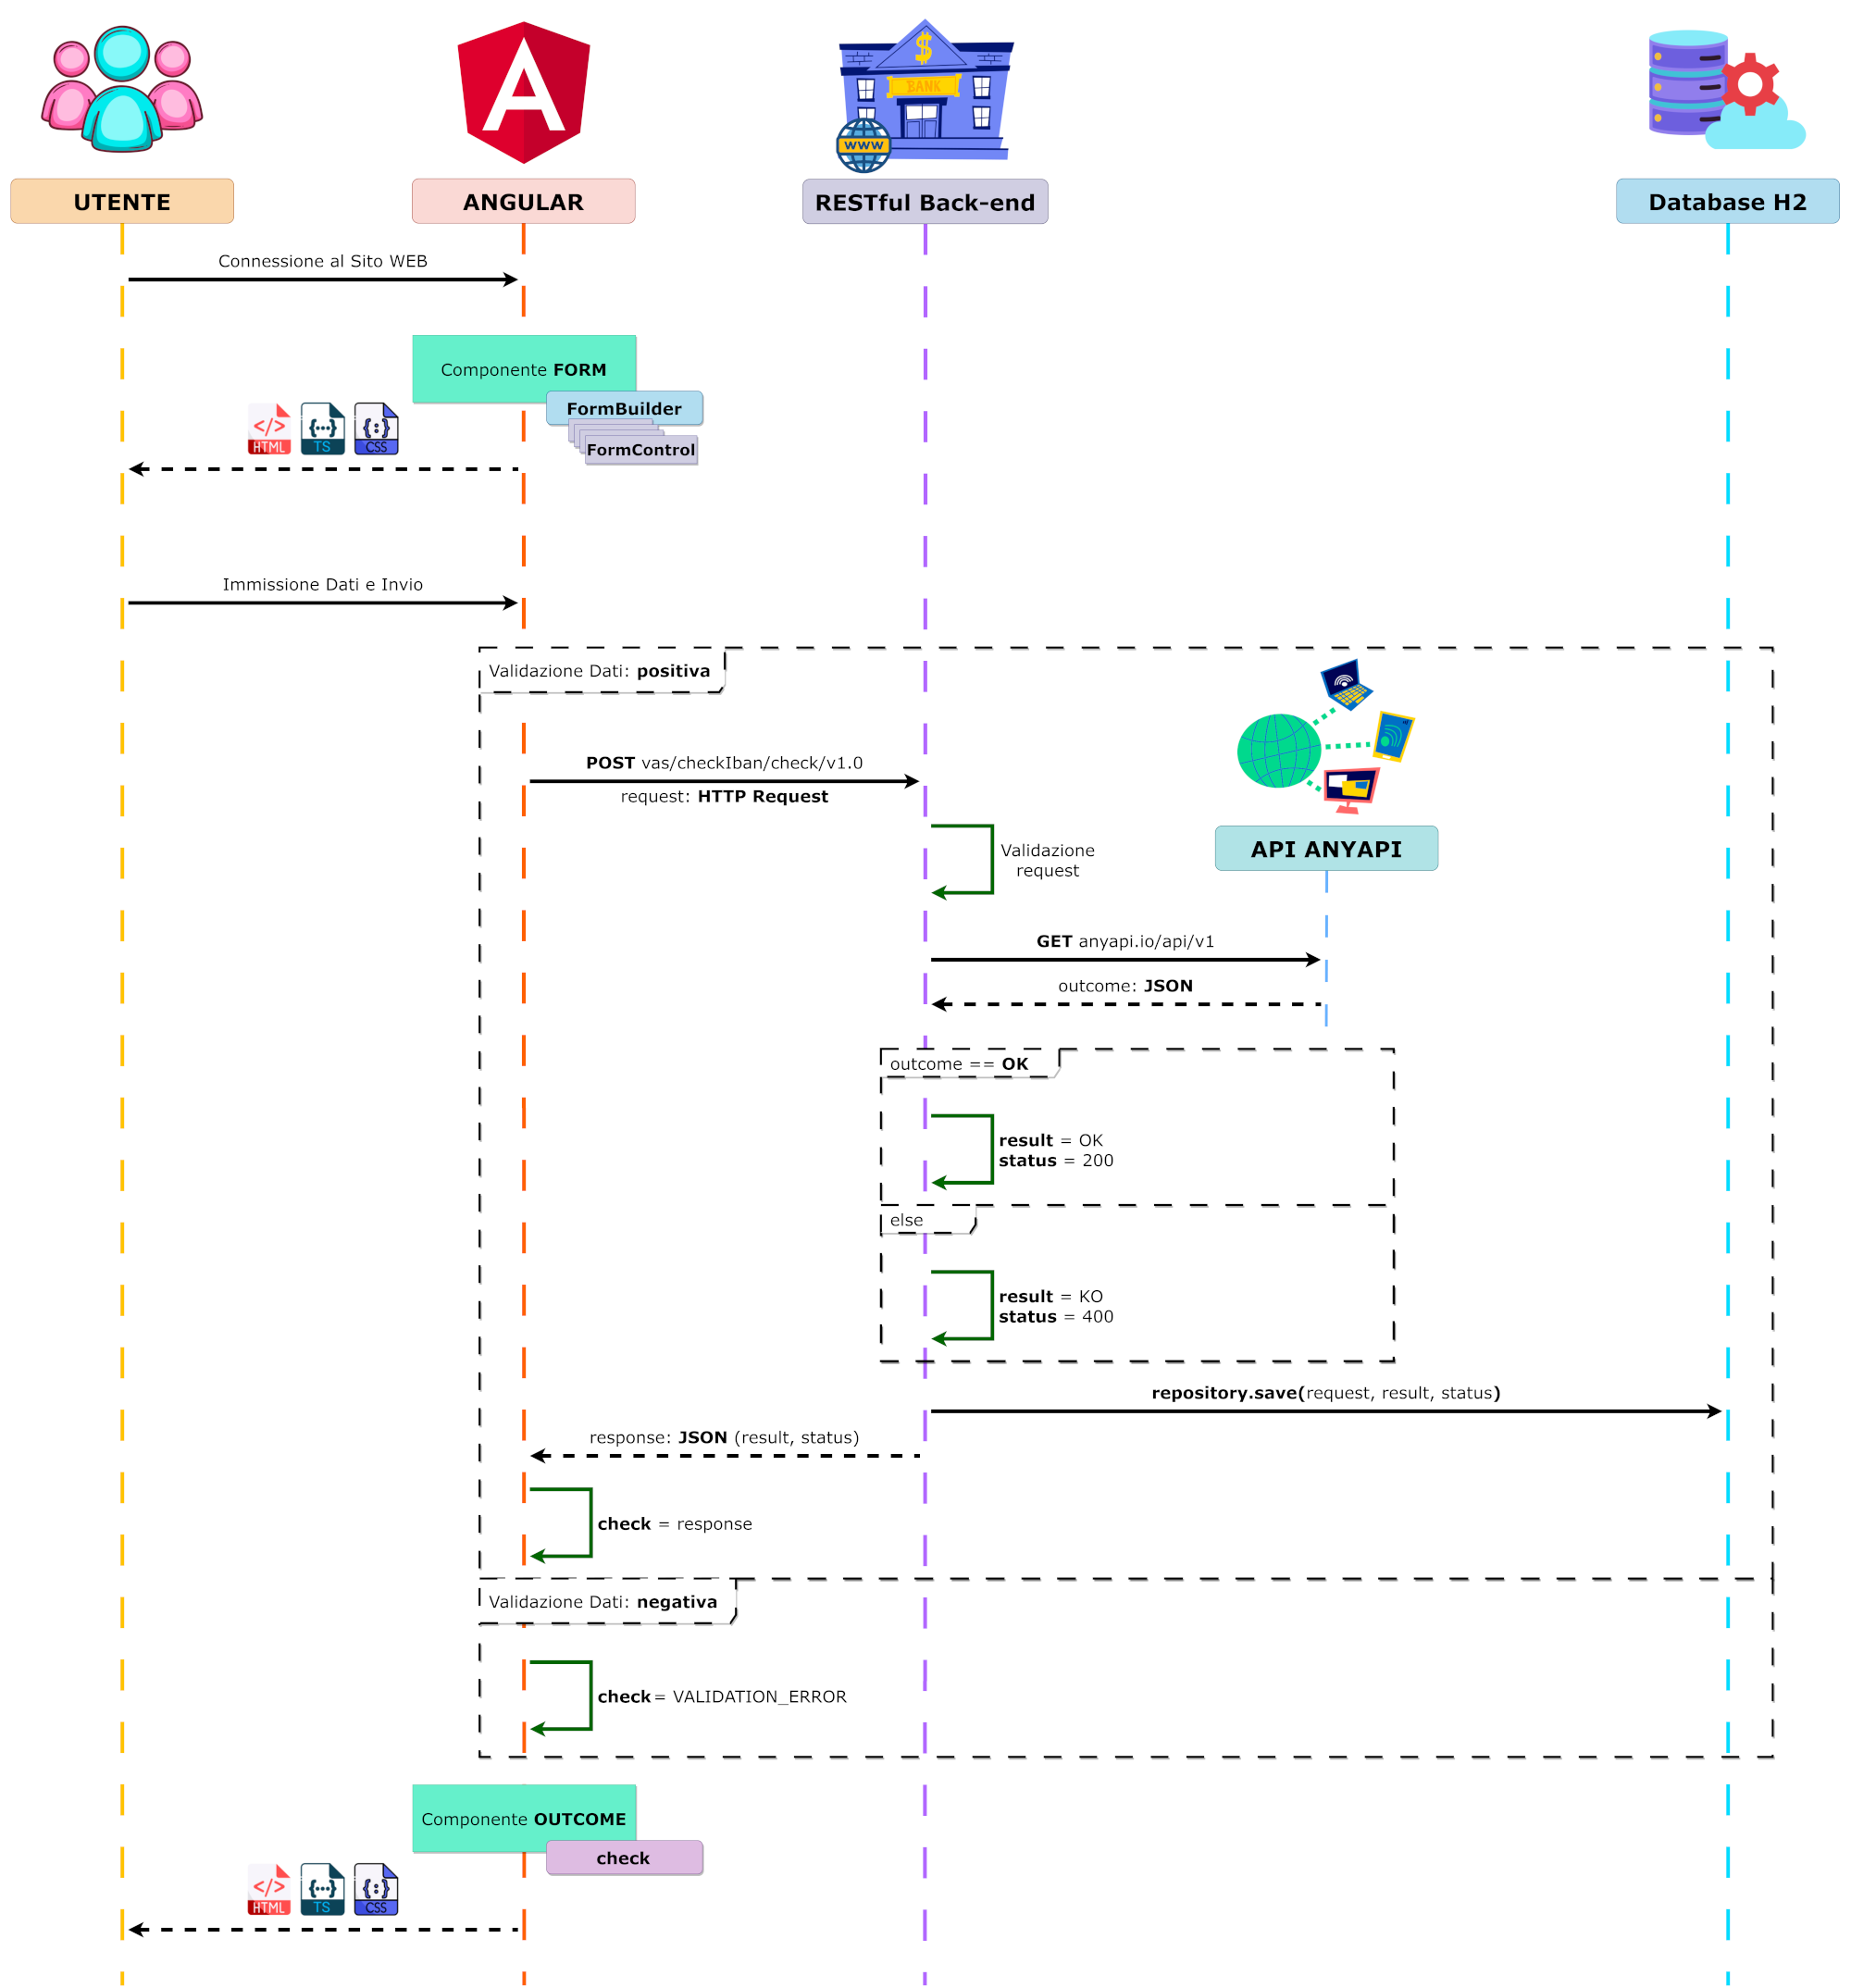
\includegraphics[width=1\textwidth]{img/Architettura.png}
  \caption{Caso d’uso principale del servizio, che comprende ogni componente realizzato e mostra le interazioni e il flusso logico dell’intera applicazione.} 
  \label{fig:Architettura.png}
\end{figure}
Il punto d’ingresso dell’applicazione è rappresentato da una \textit{web application} realizzata con il framework Angular. Il componente chiave esposto all’utente è un modulo di inserimento dati creato su misura, progettato per consentire l’inserimento accurato delle informazioni necessarie per effettuare la richiesta HTTP da inviare all’API REST fornita dal back-end. Questo modulo fornisce anche un primo livello di controllo sui dati inseriti, filtrando le informazioni per prevenire l’invio di richieste errate o dati in formati non supportati. Ciò minimizza la probabilità che il back-end interpreti erroneamente le richieste.\\
Proseguendo nell’architettura, la richiesta generata dal componente Angular viene ricevuta e processata dall’API RESTful esposta dal servizio back-end. Di seguito si illustrano i componenti e la struttura di questa sezione del progetto:
\begin{figure}[H]
  \centering
  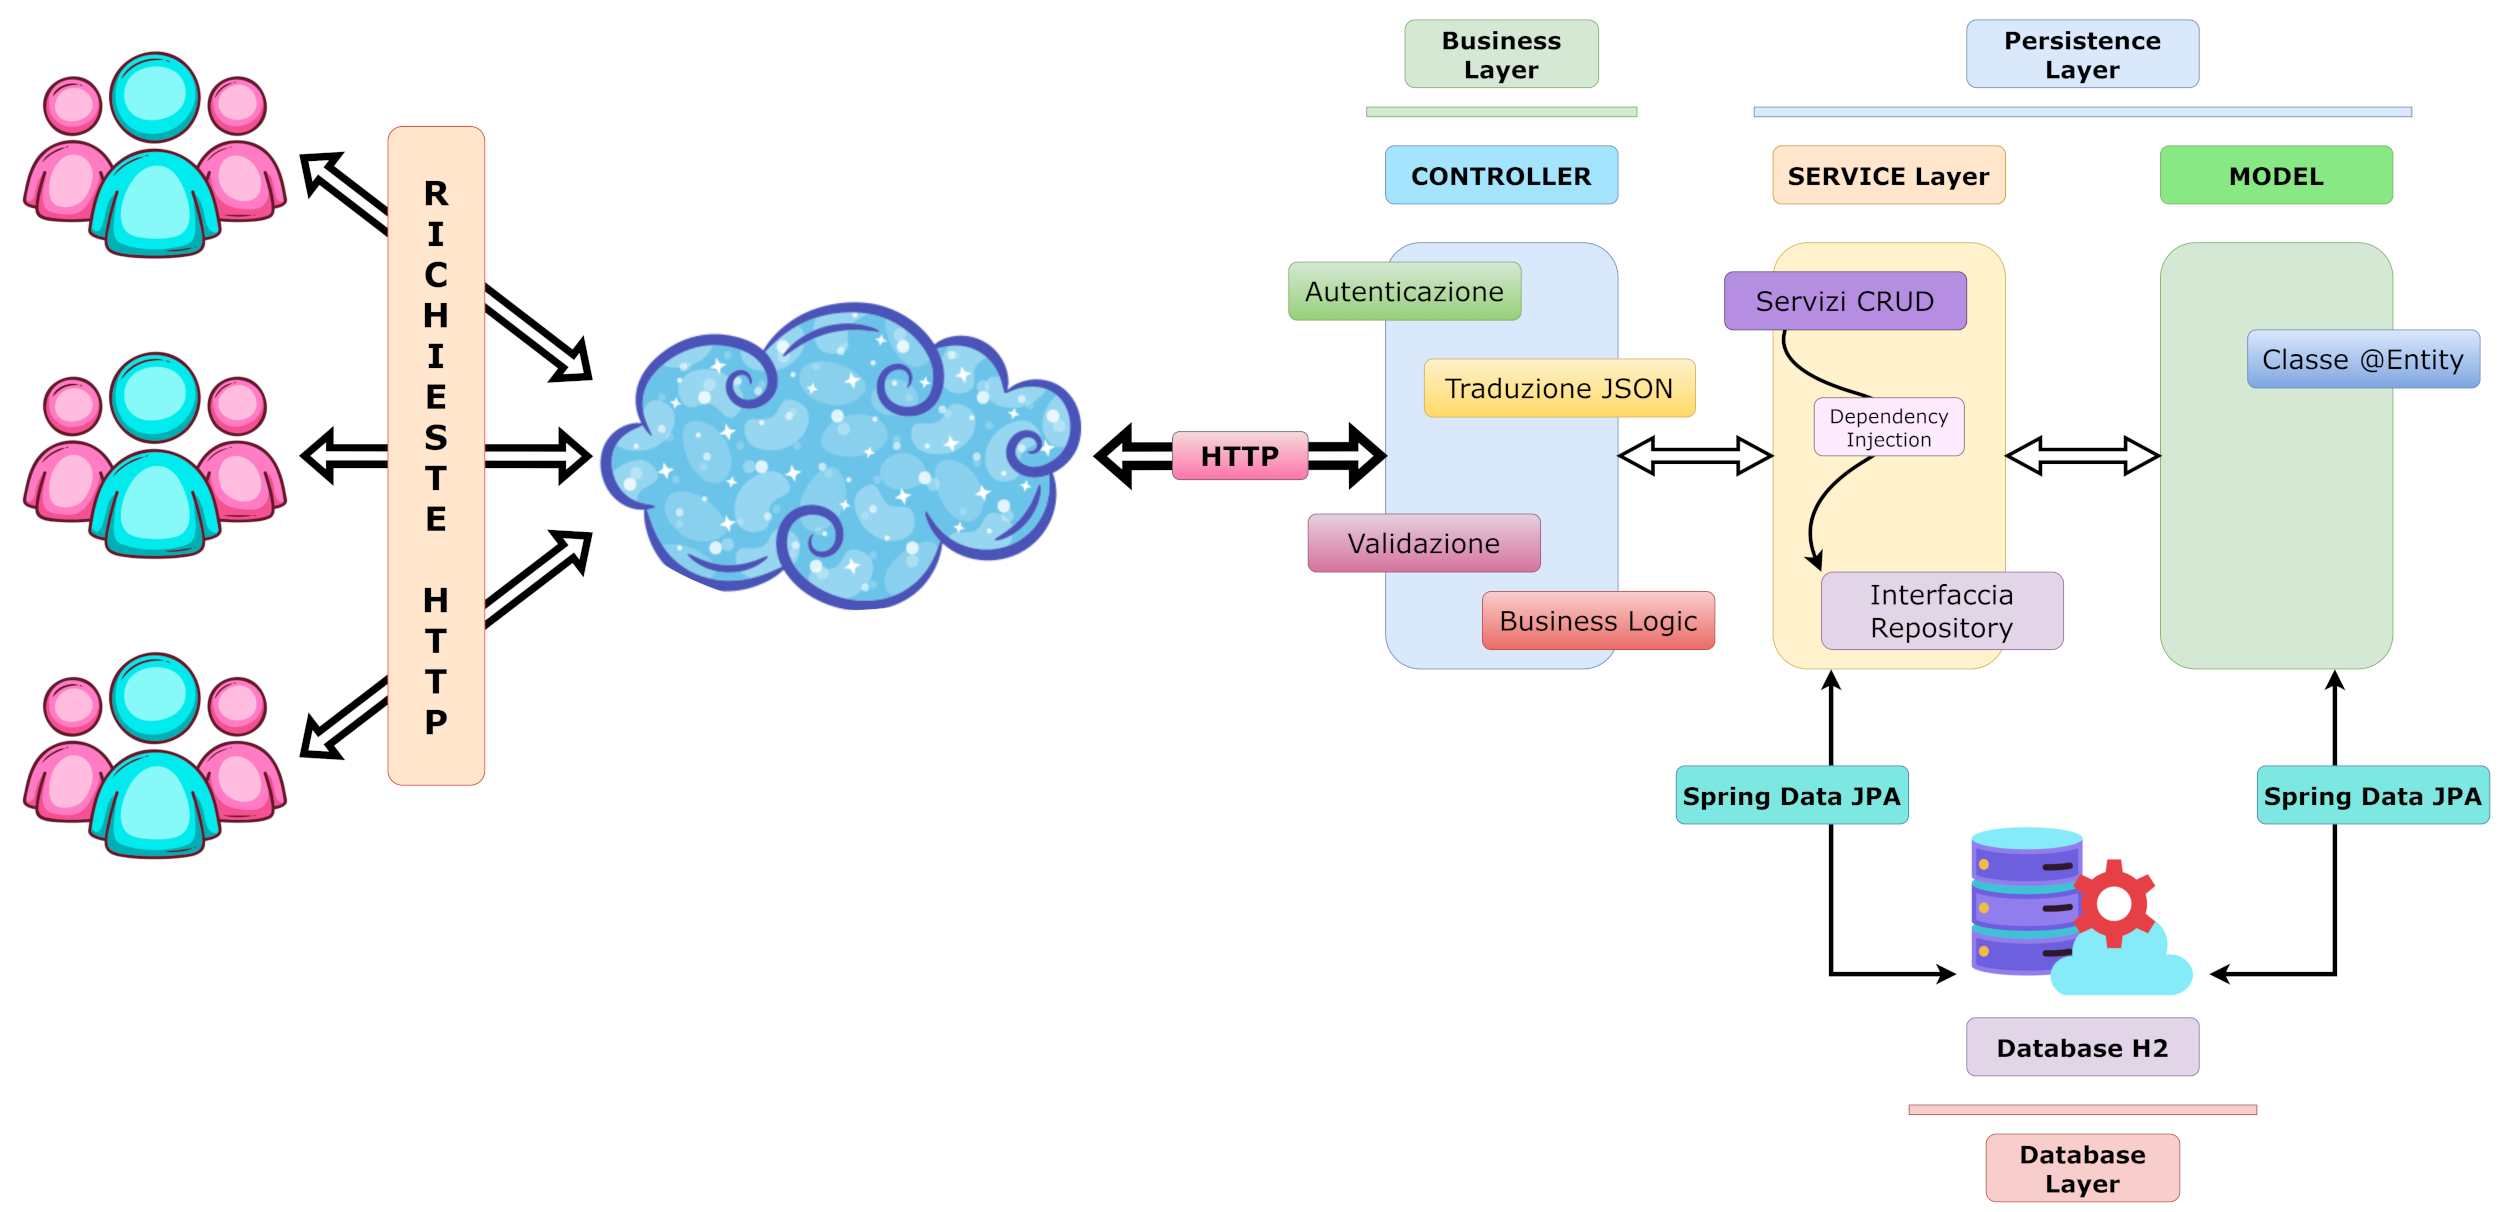
\includegraphics[width=1\textwidth]{img/SpringBoot_Diagramma.png}
  \caption{Rappresentazione dell’architettura back-end, illustrando la suddivisione logica del software e le interazioni.} 
  \label{fig:SpringBoot_Diagramma.png}
\end{figure}
Quando un \textit{client} invia una richiesta HTTP al servizio RESTful esposto dal back-end, questa viene ricevuta e gestita dal \textit{controller}, che agisce come livello di business. In questa circostanza, la richiesta viene scomposta in \textit{header} e \textit{body} e vengono prelevate le informazioni ricevute in formato JSON. Inoltre, il \textit{controller} è responsabile della gestione della logica di business dell’applicazione, come ad esempio l’elaborazione delle informazioni al fine offerto dal servizio, ovvero la validazione effettiva del codice IBAN.\\
Successivamente, avviene una transizione virtuale da livello di business a livello di persistenza, rappresentata con il passaggio dal \textit{controller} al \textit{service layer}. Questo componente logico opera sui dati mappati da Spring Data JPA con le classi del \textit{model} ed offre un’interfaccia \textit{Repository} per comunicare con il database. Oltre a ciò, il service layer consente l’applicazione della logica di archiviazione e la traduzione degli oggetti di business in righe del database e viceversa.\\
Il \textit{model}, già menzionato in precedenza, è composto dalle classi entità, che rappresentano gli oggetti Java corrispondenti alle righe del database.\\
\textit{Service layer} e \textit{model} collaborano sinergicamente per interagire con il livello di database, implementato con il DBMS H2. Sfruttando le logiche e i meccanismi messi a disposizione da Spring Data JPA, e rispettando le esigenze specifiche del database utilizzato, lo scambio di dati in entrata ed in uscita avviene in modo rapido e sicuro.\\
Infine, Spring Data fornisce annotazioni e interfacce appositamente create per agevolare l’implementazione della logica di archiviazione, consentendo agli sviluppatori di configurare rapidamente e in modo affidabile la struttura di comunicazione con il database.

\section{Back-end}

Lo sviluppo del progetto ha avuto come punto di inizio la realizzazione del servizio REST back-end, che costituisce il cuore del sistema di validazione degli IBAN. La realizzazione di questo componente, messa in pratica utilizzando il framework Spring Boot e, di conseguenza, il linguaggio di programmazione Java, ha richiesto un'attenta pianificazione, l'adozione delle migliori pratiche di sviluppo, e un'analisi dettagliata dei requisiti dell'azienda cliente.\\
Inoltre, per garantire l’integrità e la tracciabilità dei dati, è stato espressamente indicato nei requisiti di implementare un sistema di registrazione delle richieste su database H2 in-memory. Ciò ha richiesto l'utilizzo del framework Spring Data JPA per creare entità e \textit{repository} dedicati all'accesso al database, tali da garantire la persistenza delle informazioni relative alle richieste effettuate, consentendo una visione d'insieme e una possibile analisi dei dati raccolti.\\
Infine, è stato applicato il principio della testabilità tramite lo sviluppo di una suite di test automatizzati, grazie all’implementazione del \textit{tool} JUnit. Questi test hanno lo scopo di verificare la corretta funzionalità dei metodi sviluppati e di rilevare eventuali errori o \textit{bug} in modo preventivo.

\section{Servizio REST}

Come anticipato, il cuore dello sviluppo back-end dell’applicazione è l’esposizione del servizio REST basato su Spring Boot. Questo strato di servizio è responsabile per la gestione delle richieste HTTP provenienti dai \textit{client} e per la fornitura di risposte appropriate in modo efficiente e scalabile.\\
Innanzitutto, Spring Boot mette a disposizione una base solida dalla quale partire per realizzare un applicativo, generando un progetto basilare ma composto da tutte le dipendenze necessarie. Tra queste, per abilitare l'esposizione del servizio REST svolge un ruolo chiave il componente «\texttt{Spring Web}», che inoltra con precisione le richieste HTTP alle risorse dell'applicazione pertinenti e gestisce la generazione e il rilascio delle risposte ai \textit{client}, formattate come oggetti JSON. La sua integrazione abilita un flusso coerente delle richieste e delle risposte, garantendo un'esperienza utente ottimale.\\
Per quanto riguarda il processo di validazione delle richieste in arrivo, riveste una grande importanza la dipendenza «\texttt{Validation}». Questo strumento gioca un ruolo cruciale per garantire che i dati forniti dai \textit{client} rispettino le regole definite dal programmatore. In tal modo, si assicura che le richieste ricevute siano affidabili e adeguate all'elaborazione.\\
Un'altra componente vitale è «Spring Data JPA», impiegata per la persistenza dei dati relativi alle richieste. Questo componente si interfaccia direttamente con il database, consentendo la memorizzazione accurata delle informazioni sulle richieste effettuate dai \textit{client}. La possibilità di interagire con il database facilita la tracciabilità delle richieste, un requisito fondamentale per l'azienda cliente. La scelta di impiegare l'«H2 Database», un database in-memory, offre un vantaggio notevole in termini di velocità di esecuzione. Questo database, integrato nell'applicazione, garantisce un meccanismo di archiviazione efficiente e temporaneo per i dati, contribuendo così all'ottimizzazione complessiva del sistema.\\
Questi componenti collaborano per fornire un servizio affidabile e scalabile, gestendo le richieste, validando i dati in ingresso, consentendo la tracciabilità delle operazioni e garantendo un'archiviazione efficiente dei dati. L'integrazione di queste tecnologie contribuisce in modo significativo all'efficienza e alla robustezza del sistema. Inoltre, tutto questo è facilmente configurabile tramite uno strumento messo a disposizione da Spring, noto come Spring Initializr, usufruibile sia tramite l’omonimo sito web sia tramite l’estensione compatibile con tutti i principali IDE.
\begin{figure}[H]
  \centering
  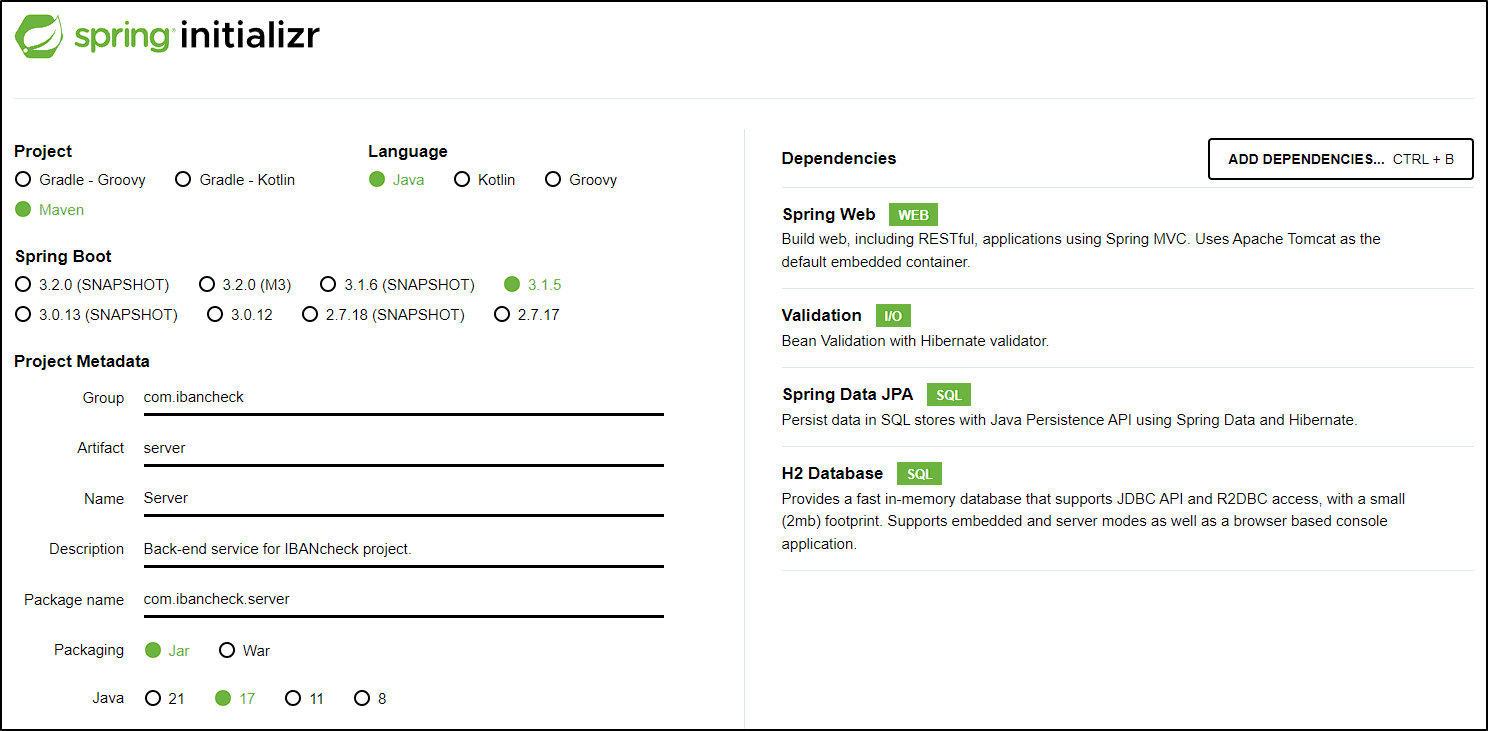
\includegraphics[width=0.9\textwidth]{img/Spring-Initializr.png}
  \caption{Configurazione iniziale del progetto e selezione delle dipendenze via Spring Initializr, da sito web.} 
  \label{fig:Spring-Initializr.png}
\end{figure}
Infine, la configurazione del programma è gestita principalmente attraverso il file \textit{pom.xml}, in cui vengono definite le dipendenze e le versioni dei linguaggi e framework usati.

\section{Controller}
Una volta scaricato il progetto configurato con Spring Initializr, è possibile aprirlo in un IDE a piacere per personalizzarne il codice sorgente e aggiungere tutte le funzionalità necessarie. Nel contesto di un servizio web REST sviluppato con Spring Boot, si semplifica l'uso del \textit{design pattern Model-View-Controller} (MVC). In questo modo, il \textit{Model} rappresenta i dati e le risorse, il \textit{Controller} coordina le richieste, mentre la \textit{View} è sostituita dalla rappresentazione dei dati inviati ai \textit{client}, tipicamente in formato JSON. Tale organizzazione offre una struttura chiara per gestire le richieste e le risposte nei servizi RESTful.\\
Per iniziare, è necessario creare una classe Java che funga da \textit{controller} e annotarla con \texttt{@RestController}, che semplifica la creazione di servizi web RESTful. Questa annotazione rappresenta una versione specializzata del \textit{controller}, combinando le funzionalità offerte da \texttt{@Controller} e \texttt{@ResponseBody}.\\
Inoltre, si aggiunge l’annotazione \texttt{@RequestMapping} per definire il percorso di base per accedere ai vari metodi esposti dalla classe. Nonostante il caso specifico preveda un \textit{controller} con attualmente un solo metodo accessibile dall'esterno, questa impostazione diventa utile se si prevede di implementare ulteriori metodi in futuro. Quindi, per il momento, si definisce il \textit{mapping} della richiesta sul percorso \texttt{vas/checkIban/check}, lasciando al singolo metodo la possibilità di specificare solo la versione del servizio:
\begin{lstlisting}[language=Java, caption=Implementazione della classe controller.]
@RestController
@RequestMapping("vas/checkIban/check")
public class ApplicationCheckController \{
		//Codice della classe...
}
\end{lstlisting}
La cosa principale da notare, per quanto mostrato finora, è l’assenza della necessità di importare manualmente le librerie nel \textit{workspace} per utilizzarle. Infatti, vengono dichiarate nel file \textit{pom.xml} in modo che Maven possa risolverle automaticamente, scaricarle ed utilizzarle per la compilazione dell’eseguibile in formato JAR.\\
Successivamente, si prosegue con la creazione del metodo principe della classe\\
\texttt{ApplicationCheckController}. Questo è responsabile di gestire le richieste di tipo POST, ricevute tramite il protocollo HTTP, che forniscono parametri sia nell’\textit{header} che nel \textit{body}.

\subsubsection{Validazione dei Dati}

Prima di poter proseguire con la validazione del codice IBAN inviato nella richiesta, è necessario verificare la correttezza dei dati forniti al servizio. Questo controllo viene effettuato in due modalità distinte, a seconda che le informazioni siano contenute nell’\textit{header} o nel \textit{body} della richiesta. Inoltre, è possibile definire il messaggio da restituire nel caso in cui il vincolo non sia soddisfatto.

\subsubsection{Parametri nell’Header}

Il caso più semplice riguarda i parametri nell’\textit{header}. È necessario specificare le proprietà che devono essere soddisfatte direttamente nella firma del metodo. Nel caso in questione, l’azienda cliente richiede di ricevere due stringhe non vuote: la prima con una lunghezza massima di 255 caratteri e la seconda di 20. La firma del metodo è quindi definita per rispettare tali requisiti:
\begin{lstlisting}[language=Java, caption=Dichiarazione dei parametri all'interno della firma del metodo.]
@RequestHeader(value = "x-request-id", required = true)
@Size(max = 255, message = "Request ID size out of range [max size = 255]") String requestId,
@RequestHeader(value = "subscriber-code", required = true)
@Size(max = 20, message = "Subscriber Code size out of range [max size = 20]") String subscriberCode
\end{lstlisting}
In questo caso, \texttt{@RequestHeader} specifica il nome del parametro presente nell’\textit{header} e fornisce l’attributo \texttt{required}. Quando impostato come nel caso attuale a \texttt{true}, rende valide solo le richieste contenenti quel parametro, escludendo stringhe vuote o nulle. Invece, l’annotazione \texttt{@Size} definisce la lunghezza delle stringhe. Nel caso in questione, è stato specificato solo l’attributo \texttt{max}, che rappresenta la lunghezza massima. Questo perché il controllo sul fatto che abbiano almeno 1 carattere è implicito nell’attributo \texttt{required} di \texttt{@RequestHeader}. Se fosse necessario avere una dimensione minima di \textit{n} caratteri, dove \textit{\texttt{n > 1}}, allora andrebbe specificato l’attributo \texttt{min} di \texttt{@Size}.

\subsubsection{Parametri nel Body}
Per quanto riguarda il \textit{body} della richiesta, la dinamica cambia leggermente. Tanto per cominciare, il tipo deve corrispondere a \texttt{JSON}, che è necessario per effettuare il \textit{parsing} in un oggetto Java, così da accedere ai dati contenuti. Questo viene realizzato attraverso la creazione di un oggetto \texttt{Provider} che riflette la struttura del JSON, seguito dall’impostazione dei vincoli di validità sugli attributi.
\begin{lstlisting}[language=Java, caption=Dichiarazione dei vincoli di validità per i dati contenuti nel \textit{body} della richiesta.]
@NotNull(message = "Provider Code cannot be null")
@Size(max = 20, message = "Provider Code size out of range [max size = 20]")
private String providerCode;
@NotNull(message = "Account ID cannot be null")
@Size(max = 34, message = "Account ID size out of range [max size = 34]")
@Pattern(regexp = "[A-Z]{2}[0-9]{2}[A-Z0-9]{1,30}|[A-Z0-9]{1,30}", message = "Account ID has invalid format")
private String accountId;
@Size(max = 16, message = "Tax Code size out of range [max size = 16]")
@Pattern(regexp = "([0-9a-zA-Z-+/]){0,16}", message = "Tax Code has invalid format")
private String taxCode;
@Size(max = 14, message = "Vat Code size out of range [max size = 14]")
@Pattern(regexp = "([0-9a-zA-Z]){0,14}", message = "Vat Code has invalid format")
private String vatCode;
\end{lstlisting}
In questo contesto, le informazioni obbligatorie consistono in \texttt{providerCode} e \texttt{accountId}, che sono gli unici attributi annotati con il vincolo \texttt{@NotNull}. Gli altri due attributi sono opzionali e, pertanto, non sono stati sottoposti alla stessa annotazione. Alcuni attributi presentano inoltre l’annotazione \texttt{@Pattern}, che specifica il \textit{pattern} che devono rispettare per poter essere considerati validi, basandosi su espressioni regolari.Il tag \texttt{@Size} opera in modo analogo a quanto visto per gli attributi nell’\textit{header}.\\
Una volta fatto ciò, il processo non è ancora concluso. All’interno del metodo del \textit{controller} in cui viene ricevuta la richiesta, è fondamentale indicare che il JSON deve essere convertito in un oggetto \texttt{Provider} e che i suoi attributi devono essere validati. Quindi, si dichiara il parametro nel metodo come \texttt{@Valid @RequestBody Provider}, affinché Spring identifichi quell’oggetto come la rappresentazione del JSON nel \textit{body} e ne effettui la validazione in base alle regole interne. Infine, per specificare il consumo di un JSON, il metodo è annotato con \texttt{@PostMapping(path = "/v1.0", consumes = "application/json", produces = "application/json")}. Ciò indica il percorso (\texttt{path}) specifico del metodo, il tipo di input proveniente dal \textit{body} ed il tipo di risposta restituito.

\subsection{Comunicazione con API Esterna}

Una volta validati tutti i dati necessari al servizio, si procede con il controllo del codice IBAN inserito per verificarne la correttezza. Tale procedura si basa sull’uso di un’API esterna fornita da \href{http://anyapi.io/}{anyapi.io}, con cui si stabilisce comunicazione direttamente dal \textit{controller}.

\subsubsection{Creazione del Data Transfer Object}

Per iniziare questa fase, si crea il \textit{Data Transfer Object} (DTO), un oggetto Java usato per lo scambio di dati, impiegato per mappare la risposta ottenuta dall’API esterna. A tal fine, è fondamentale comprendere la struttura della risposta fornita dal servizio \textit{anyapi}. In particolare, si tratta di un JSON del seguente formato:
\begin{lstlisting}[caption=Struttura del JSON restituito dall'API esterna.]
{   "valid": true,
    "iban": "BE68 5390 0754 7034",
    "countryCode": "BE",
    "bban": "539007547034",
    "electronicFormat": "BE68539007547034"   }
\end{lstlisting}
Ora che si conosce la struttura della risposta, bisogna creare una classe con attributi corrispondenti ai campi del JSON. Affinché la mappatura possa avvenire correttamente, è essenziale fornire i metodi \textit{getter} e \textit{setter} per ogni attributo. Inoltre, la classe deve implementare l’interfaccia \texttt{Serializable}; altrimenti, non potrebbe essere utilizzata negli scambi HTTP, e dunque non sarebbe di fatto un \textit{Data Transfer Object}. La classe risultante è la seguente:
\begin{lstlisting}[language=Java, caption=Classe \textit{Data Transfer Object} utilizzata per mappare la risposta dell'API esterna.]
public class Iban implements Serializable {
    private String iban;
    private boolean valid;
    private String countryCode;
    private String bban;
    private String electronicFormat;

    public Iban() {
    }
	// getter e setter...
}
\end{lstlisting}

\subsubsection{Utilizzo delle Informazioni da application.properties}

Al fine di migliorare la leggibilità e la coesione del codice, oltre ad agevolare l’individuazione delle variabili che contengono il \textit{link} e la chiave dell’API esterna, è stato scelto di collocare questi valori all’interno del file di configurazione \textit{application.properties}. A tal proposito, sono state create due variabili:
\begin{lstlisting}[caption=Dichiarazione delle variabili all'interno del file di configurazione.]
anyapi.api_key = ---chiave-api---
anyapi.url_template = https://anyapi.io/api/v1/iban?iban=%s&apiKey=%s
\end{lstlisting}
Nel codice, il \textit{controller} è annotato con \texttt{@PropertySource(value = \\"classpath:application.properties")}, specificando così il file di configurazione in cui effettuare la ricerca. Successivamente, vengono definite due variabili interne di tipo stringa:
\begin{itemize}
    \item \texttt{API\_KEY}
    \item \texttt{URL\_TEMPLATE}
\end{itemize}
Inoltre, è presente una variabile d’ambiente denominata \texttt{env}, di tipo \\\texttt{org.springframework.core.env.Environment}. Questa variabile è annotata con \\\texttt{@Autowired} e dev’essere privata, permettendo a Spring di iniettare automaticamente le dipendenze cercando un \textit{bean} gestito dal \textit{container} che corrisponda a quel tipo di dato (\texttt{Environment}), assegnandolo all’attributo. Infine, si utilizza il metodo \texttt{getProperty} di \texttt{env} per accedere al file di configurazione e recuperare il valore corrispondente, specificando il nome della variabile contenuta in \textit{application.properties}:
\begin{lstlisting}[language=Java, caption=Recupero delle informazioni per effettuare la chiamata all'API.]
API_KEY = env.getProperty("anyapi.api_key");
URL_TEMPLATE = env.getProperty("anyapi.url_template");
\end{lstlisting}

\subsubsection{Richiesta verso API Esterna}

Per avviare il processo di richiesta, una fase chiave coinvolge l'importazione della classe \texttt{org.springframework.web.client.RestTemplate}, che svolge un ruolo fondamentale nella comunicazione con le API esterne permettendo di effettuare richieste HTTP sincrone. Una volta dichiarata e istanziata una variabile di tipo \texttt{RestTemplate}, è possibile utilizzare il metodo \texttt{getForObject(String url, Class responseType)} per iniziare una richiesta HTTP di tipo \texttt{GET} all'URL specificato.\\
Questo metodo richiede due parametri principali:
\begin{enumerate}
    \item \textbf{\texttt{url}}: è l’indirizzo di destinazione, composto tenendo conto delle informazioni raccolte nella sezione antecedente.
    \item \textbf{\texttt{responseType}}: rappresenta la classe Java in cui si desidera convertire la risposta HTTP ricevuta dall'API esterna e corrisponde al \textit{Data Transfer Object} realizzato in precedenza.
\end{enumerate}
Si sottolinea che in caso di errore durante la richiesta, il metodo \texttt{getForObject} restituisce un valore \texttt{null}. Pertanto, è fondamentale eseguire un controllo immediatamente dopo la chiamata per verificare se l'oggetto risultante è stato popolato correttamente. Questa verifica è necessaria per confermare che la richiesta sia stata completata con successo. Nel caso in cui l'oggetto sia nullo, è fondamentale gestire l'errore in modo adeguato, stabilendo procedure di gestione degli errori in grado di garantire un comportamento affidabile da parte del sistema.

\section{Database}

Uno degli obiettivi principali del progetto è il tracciamento delle richieste al servizio di validazione dei codici IBAN. A tale scopo, è stato adottato un approccio che dà priorità alla velocità di esecuzione a discapito della memoria utilizzabile. Ciò è motivato dalla previsione iniziale di un basso numero di richieste. Pertanto, è stata scelta l’opzione di utilizzare un database in-memory conosciuto come H2.

\subsection{Schema SQL}
Anche in questa circostanza, il framework Spring, specialmente Spring Data, si rivela estremamente utile ed affidabile. Una volta integrate le dipendenze nel file \textit{pom.xml}, che grazie a Maven permette di scaricare ed utilizzare le librerie all’interno del progetto, è sufficiente definire un file SQL con lo scheletro della tabella da realizzare. Automaticamente , Spring implementa il database H2 secondo lo schema:
\begin{lstlisting}[language=SQL, caption=Schema SQL per la tracciatura delle richieste.]
DROP TABLE VALIDATION_LOGS IF EXISTS;
CREATE TABLE VALIDATION_LOGS (
    request_id VARCHAR(255) PRIMARY KEY,
    subscriber_code VARCHAR(20) NOT NULL,
    provider_code VARCHAR(20),
    response_code BIGINT NOT NULL,
    outcome VARCHAR(255) NOT NULL,
    error VARCHAR(255),
    iban_validated VARCHAR(255) NOT NULL,
    request_timestamp TIMESTAMP NOT NULL,
    response_timestamp TIMESTAMP NOT NULL
)
\end{lstlisting}
In questo caso, è importante precisare che, qualora non venga specificato un file SQL contenente lo schema per il database, Spring è in grado di crearne uno basandosi sulla classe (o eventuali più classi) annotata con \texttt{@Entity}.

\subsection{Entità}
Affinché Spring Data JPA possa mappare una classe ad una tabella del database, è necessario annotarla come entità. Inoltre, questa classe, chiamata in gergo tecnico POJO, deve avere un costruttore privo di argomenti ed un attributo che rappresenta la chiave primaria nella relativa tabella. A tale scopo, è stata implementata una classe chiamata \texttt{Persistence}, che funge da entità, in cui l’attributo \texttt{requestId} rappresenta la chiave primaria:
\begin{lstlisting}[language=Java, caption=Implementazione della classe entità.]
@Entity
@Table(name = "VALIDATION_LOGS")
public class Persistence {
    @Id
    @Column(name = "request_id", length = 255)
    private String requestId;
    @Column(name = "subscriber_code", nullable = false, length = 20)
    private String subscriberCode;
    @Column(name = "provider_code", nullable = true, length = 20)
    private String providerCode;
    @Column(name = "response_code", nullable = false, length = 3)
    private int responseCode;
    @Column(name = "error", nullable = true, length = 21)
    private String error;
    @Column(name = "outcome", nullable = false, length = 2)
    private String outcome;
    @Column(name = "iban_validated", nullable = false, length = 255)
    private String ibanValidated;
    @Column(name = "request_timestamp", nullable = false)
    @Temporal(TemporalType.TIMESTAMP)
    private Date requestTimestamp;
    @Column(name = "response_timestamp", nullable = false)
    @Temporal(TemporalType.TIMESTAMP)
    private Date responseTimestamp;

    public Persistence() {
    }
		// codice di getter e setter...
}
\end{lstlisting}
Esaminando l’implementazione dell’entità, emergono alcune particolarità:
\begin{itemize}
    \item Oltre ad essere annotata con \texttt{@Entity}, la classe è stata decorata con \texttt{@Table}. Questo per specificare il nome della tabella nel database che deve corrispondere all’entità, poiché nello schema SQL precedentemente esaminato abbiamo assegnato un nome diverso alla tabella rispetto a quello della classe entità.
    \item La chiave primaria della classe è annotata con \texttt{@Id}.
    \item Ogni attributo è annotato con \texttt{@Column}, che definisce il nome della colonna a cui corrisponde quell’attributo. In alcuni casi, definisce anche la lunghezza massima che può assumere un attributo e se può essere \texttt{null} oppure no. Questo consente una validazione preventiva prima che un oggetto venga salvato nel database, facilitando la rilevazione di errori prima della persistenza effettiva.
    \item I due attributi di tipo \texttt{Date} sono annotati con \texttt{@Temporal} per specificare il tipo di valore temporale a cui corrispondono. Naturalmente, questi valori devono coincidere con quelli definiti nello schema SQL.
\end{itemize}

\subsection{Repository}

Giunti a questo punto, sono disponibili tutti gli elementi necessari per stabilire un collegamento tra la tabella del database e l’entità Java. Vediamo come rendere effettiva questa comunicazione.\\
Spring Data JPA si concentra sull'utilizzo di JPA per salvare dati in database relazionali. La sua funzionalità più principale in quest’ambito è la capacità di creare automaticamente implementazioni di \textit{repository}, a runtime, partendo dalla definizione di un'interfaccia, chiamata appunto \textit{repository}. Quindi, è necessario creare un’interfaccia denominata \texttt{PersistenceRepository}, in grado di operare con entità \texttt{Persistence}:
\begin{lstlisting}[language=Java, caption=Implementazione dell'interfaccia Repository.]
public interface PersistenceRepository extends CrudRepository<Persistence, String> {
    Persistence findByRequestId(String requestId);
    List<Persistence> findBySubscriberCode(String subscriberCode);
    List<Persistence> findByProviderCode(String providerCode);
}
\end{lstlisting}
Innanzitutto, si osserva l’estensione di un’altra interfaccia, \texttt{CrudRepository}, che consente di specificare (attraverso i due parametri generici) il tipo dell’entità con cui operare ed il tipo di identificatore da utilizzare. Come specificato precedentemente, non è necessario definire una classe che implementi \texttt{PersistenceRepository} per usare i metodi qui definiti: Spring Data JPA si occupa di tutto in modo autonomo. Pertanto, è possibile definire tutti i metodi desiderati all’interno di questa interfaccia, per recuperare dati o persistere informazioni nel database. Successivamente, il framework farà assunzioni sulla firma dei metodi per garantire il corretto funzionamento di ciascuno.\\
Una volta completati questi passaggi, è possibile richiamare uno qualsiasi dei metodi definiti in \texttt{PersistenceRepository} o nell’interfaccia estesa \texttt{CrudRepository} per comunicare col database. Nel \textit{controller} dell’applicazione, quando arriva una nuova richiesta, la prima azione è verificare che l’\texttt{id} non sia già presente nel database. In caso affermativo, viene restituito immediatamente un errore. Per fare ciò, viene richiamato il metodo \texttt{findByRequestId(requestId)}.

\section{Front-end}

Il front-end dell’applicazione si basa interamente sul framework di sviluppo Angular, utilizzato per creare l’interfaccia utente dell’applicazione come \textit{Single Page Application}. La \textit{web application} è stata realizzata focalizzandosi sulla creazione e la comunicazione dei componenti, resa possibile da fondamentali script TypeScript, utilizzati anche per la presentazione dell’output nella pagina.

\section{Angular Web-Application}
L’architettura software di una \textit{web application} Angular è cruciale per garantire una struttura ben organizzata e scalabile del progetto. Infatti, una delle caratteristiche principali di questo framework è la modularità, che favorisce la suddivisione dell’applicativo e la comunicazione tra i vari componenti seguendo il \textit{pattern} architetturale MVC. Inoltre, Angular offre una vasta gamma di librerie e pacchetti che agevolano l’interazione con i servizi back-end, consentendo all’applicazione di recuperare le informazioni necessarie in tempo reale e di gestire le operazioni in modo sicuro.\\
Per iniziare a sviluppare un'applicazione Angular, è essenziale possedere anche Node.js e NPM. Senza entrare troppo nei dettagli, il primo offre un ambiente di esecuzione per il codice JavaScript, mentre il secondo è un registro di software \textit{open-source} per la gestione dei pacchetti. Nel caso in esame, NPM serve per recuperare il \textit{package} Angular CLI, che consente di creare un \textit{workspace} Angular con il comando \texttt{ng new <nome\_progetto>}, dove il nome del progetto corrisponde a \texttt{iban-check}.

\section{Componenti}

Nel contesto Angular, con il termine «componenti» si fa riferimento ai blocchi che compongono un’applicazione. Ogni componente è costituito da una classe TypeScript decorata con \texttt{@Component()}, un template HTML e degli stili CSS che definiscono l’aspetto degli elementi del template. Questi componenti possono essere creati utilizzando il comando \texttt{ng generate component <nome\_componente>} tramite Angular CLI.
Nel caso in esame, la \textit{web application} è formata da 4 componenti:
\begin{enumerate}
    \item \textbf{form} → rappresenta il modulo per l’inserimento dei dati;
    \item \textbf{offline} → costituisce la schermata da visualizzare se il servizio back-end non è raggiungibile;
    \item \textbf{outcome} → mostra il risultato dell’elaborazione del back-end;
    \item \textbf{top-bar} → è la barra superiore, presente in ogni schermata dell’applicazione.
\end{enumerate}
I componenti Angular sono il cuore dell'applicazione. Ognuno di essi è responsabile di un aspetto specifico dell'interfaccia utente e della logica di presentazione dei dati. Come esposto in precedenza, l'architettura software promuove la separazione dei compiti e la riutilizzabilità del codice attraverso la modularità. La comunicazione tra i componenti avviene tramite i servizi Angular e l'emissione di eventi personalizzati. Questa struttura permette di mantenere il codice più manutenibile e facilita lo sviluppo di front-end caratterizzati da un’interazione con l’utente complessa.

\subsection{Form di Immissione}

La pagina principale dell’applicazione, nonché il punto in cui l’utente inserisce i propri dati nel sistema, è rappresentata dal componente \texttt{form}. Come ogni componente, possiede un template HTML ed un file TypeScript, che contiene la logica e la definizione dei campi.
L’elemento \texttt{<form>} nel file HTML è legato ad un \texttt{FormGroup} presente nello script, in modo da effettuare direttamente la validazione dei campi:
\begin{lstlisting}[language=HTML, caption=\textit{Binding} dell'elemento \texttt{form} tra HTML e TypeScript.]
<form [formGroup]="ibanCheckForm">
\end{lstlisting}
All’interno del file TypeScript, il \texttt{FormGroup} è associato ad un \texttt{FormBuilder} ed ogni campo è rappresentato da un oggetto \texttt{FormControl}. In questo modo, è possibile implementare la validazione e definire il controllo automatico dei valori, così che l’applicazione eviti di effettuare richieste contenenti dati sintatticamente errati.
\begin{lstlisting}[language=Java, caption=Codice TypeScript che realizza la validazione di alcuni campi del \texttt{form}.]
ibanCheckForm = this.formBuilder.group({
    subscriberCode: new FormControl('', [Validators.required, Validators.maxLength(20)]),
    accountId: new FormControl('', [Validators.required, Validators.maxLength(34), Validators.pattern("[A-Z]{2}[0-9]{2}[A-Z0-9]
          {1,30}|[A-Z0-9]{1,30}")])
    
    // Proprieta' di validazione degli altri campi...
});
\end{lstlisting}

\subsection{Chiamata a Back-end}

All’interno di un’applicazione web Angular, la chiamata al servizio back-end rappresenta un passaggio fondamentale, poiché consente di scambiare dati con il lato server e ricevere risposte che influenzano l’esperienza dell’utente.\\
Il componente che gestisce questa comunicazione è essenziale per l’interazione tra l’applicazione front-end ed il servizio back-end, e nel caso del progetto attuale è rappresentato da \texttt{form}. In generale, il componente designato svolge un ruolo cruciale nella preparazione dei dati per la chiamata, eseguendo la validazione dei valori inseriti dall’utente, come analizzato nella sezione precedente.\\
Una volta fatto ciò, le informazioni vengono mappate per creare \textit{header} e \textit{body} della richiesta HTTP da inoltrare al back-end. A questo punto, possono verificarsi 3 scenari:
\begin{enumerate}
    \item Il servizio back-end è offline o non raggiungibile.
    \item L’elaborazione non ha avuto successo e la risposta del servizio back-end contiene un errore.
    \item L’elaborazione ha avuto successo e la risposta del servizio back-end contiene un valore.
\end{enumerate}
In ogni caso, la chiamata avviene utilizzando un oggetto di tipo \texttt{HttpClient}, classe iniettata da Angular che consente di effettuare richieste HTTP. In particolare, la richiesta attuale è una \texttt{POST} così composta:
\begin{lstlisting}[language=Java, caption=Codice TypeScript per la preparazione di una chiamata su protocollo HTTP.]
this.http.post<Outcome>('http://localhost:8080/vas/checkIban
  /check/v1.0', body, httpOptions).pipe(retry(0), catchError((error: HttpErrorResponse) => {
    if (error.status === 0) {
        console.error('An error occurred:', error.error);
        this.activeLoading = !this.activeLoading;
        this.offNotify.emit();
    } else {
        console.error("Backend returned code " + error.status + ", body was: ", error.error);
        this.saveAndNotify(accCode, subCode, error.error);
    }    
    this.outcome = "Error";
    return throwError(() => Error("Errore rilevato!"));
    }));
\end{lstlisting}
Quindi, si analizzano le operazioni principali, ovvero:
\begin{itemize}
    \item L’interfaccia \texttt{Outcome}, realizzata appositamente per il progetto, consente di mappare automaticamente il corpo della risposta del back-end in un oggetto TypeScript.
    \item L'uso dell'operatore \texttt{pipe}, fondamentale per creare una \textit{pipe} asincrona attraverso la quale vengono passati i dati mappati.
    \item L'operatore \texttt{retry}, per specificare quante volte riprovare la richiesta in caso di fallimento, prima di ritirarsi.
    \item L'operatore \texttt{catchError}, che cattura eventuali errori contenuti nella risposta HTTP. In particolare, se il codice di stato dell'errore è \texttt{0} allora viene segnalato che il back-end o il dispositivo utente è offline. In caso contrario, si analizza il valore ricevuto dal back-end e lo si comunica all'utente.
\end{itemize}
Oltre a ciò, il componente è in grado di comunicare con gli altri attraverso due metodi: \texttt{offNotify.emit()} e \texttt{saveAndNotify()}. Il primo è usato per notificare agli altri componenti che il servizio back-end non è raggiungibile, mentre il secondo per notificare la ricezione di una risposta, attivando le schermate adeguate per comunicare l’evento all’utente.\\
Per completare correttamente la chiamata al back-end, l’oggetto \texttt{Observable} restituito dalla \textit{pipe} deve essere sottoscritto utilizzando il metodo \texttt{subscribe}. In questa circostanza, si può richiamare una funzione \textit{lambda} che riceve i dati restituiti dalla chiamata e li processa secondo le logiche del caso:
\begin{lstlisting}[language=Java, caption=Sottoscrizione della chiamata HTTP verso il back-end.]
checkIbanPost.subscribe((data: Outcome) => this.saveAndNotify(accCode, subCode, data));
\end{lstlisting}
La capacità di gestire errori e la gestione dei dati ricevuti dai servizi contattati permettono di fornire un’esperienza utente completa e scorrevole. Questa struttura, è fondamentale affinché i dati vengano correttamente scambiati tra il front-end e il back-end delle applicazioni web.

\subsection{Comunicazione tra Componenti}

Finora è stata menzionata più volte la comunicazione tra componenti, poiché è un aspetto fondamentale delle applicazioni Angular. Si tratta di una funzionalità che consente la creazione di un'esperienza utente coesa e interattiva, utilizzata nel contesto attuale per trasmettere i dati della risposta del servizio back-end dal componente \texttt{form} ai componenti \texttt{outcome} o \texttt{offline}.\\
Questo processo si basa su due elementi chiave: \texttt{Output} ed \texttt{Input}. Esaminiamo in dettaglio l'architettura e il funzionamento di tale processo di comunicazione.

\subsubsection{Emettere un Evento}
All’interno del file TypeScript del componente che emette la notifica, viene implementato un attributo chiamato \texttt{notify}. Questo elemento ha tipo \texttt{EventEmitter} ed è decorato con \texttt{@Output}, annotazione che identifica una proprietà di output in grado di emettere eventi personalizzati.\\
Una volta configurato l’attributo, è possibile utilizzare il metodo \texttt{emit()} per inviare le informazioni necessarie al componente che riceve l’evento. Questo processo è essenziale per la trasmissione di dati tra i vari componenti all’interno dell’applicazione.\\
A livello più alto, il componente mittente è dichiarato nel codice HTML con una proprietà particolare:
\begin{lstlisting}[language=HTML, caption=Dichiarazione di un componente in grado di notificare eventi.]
<app-form [ngClass]="activeForm ? 'active' : ''" (notify)="onNotify($event)"></app-form>
\end{lstlisting}
Come si evince dal codice, ci si aspetta che, ad un certo punto, un campo chiamato \texttt{notify} emetta un evento all’interno del componente \texttt{form}. Quando questo avviene, l’evento viene catturato e gestito dalla funzione indicata, ossia \texttt{onNotify}.

\subsubsection{Ricevere un Evento}
Alla funzione \texttt{onNotify} del componente padre viene passato un parametro opzionale, ovvero che può essere non specificato al momento di emissione dell’evento. Nel nostro caso, se presente, rappresenta l’esito della validazione back-end del codice IBAN inviato dall’utente. Successivamente, il metodo è strutturato per modificare la vista attiva, permettendo la visualizzazione del risultato:
\begin{lstlisting}[language=Java, caption=Funzione richiamata quando viene ricevuto un evento.]
onNotify(out?: Outcome) {
  if (out !== null && out !== undefined)
    this.outcome = out;
  invertActiveOutput();
}
\end{lstlisting}
Una volta abilitata la vista corretta, viene mostrato il componente \texttt{outcome}, così definito nel codice HTML:
\begin{lstlisting}[language=HTML, caption=Dichiarazione del componente attivato in seguito alla ricezione di un evento.]
<app-outcome [ngClass]="activeOutcome ? 'active' : ''" [outcome]="outcome"></app-outcome>
\end{lstlisting}
In questo caso, viene realizzato il \textit{binding} del campo \texttt{outcome} con l’omonimo attributo all’interno del file di TypeScript del componente.
\newpage
Infatti, nello script si trova il secondo elemento che è stato menzionato inizialmente, ovvero \texttt{Input}:
\begin{lstlisting}[language=Java, caption=Dichiarazione di un campo che riceve il proprio valore dal componente padre.]
@Input() outcome: Outcome | undefined;
\end{lstlisting}
Questa annotazione indica che il valore della proprietà è ricevuto direttamente dal componente padre. Infatti, si riflette il fatto che questo campo sia opzionale, proprio come il parametro della funzione \texttt{onNotify} esaminata in precedenza.\\
Inoltre, dal codice HTML del componente si è in grado di accedere direttamente al valore del campo. Quindi, attraverso l’uso delle direttive \texttt{NgIf}, è possibile definire condizioni per mostrare diversi contenuti basati sulla presenza o sull'assenza di dati in un oggetto opzionale, proprio come nel caso corrente. Questo permette una gestione dinamica della visualizzazione delle informazioni all’utente.\\
Infine, tutti i componenti dell’applicazione comunicano in modo simile a quanto visto finora. Questo approccio di comunicazione standardizzato agevola la manutenibilità e la scalabilità delle applicazioni, rendendo Angular uno dei migliori framework per la realizzazione di applicazioni web moderne.
\chapter{Conclusioni}
\label{chap:Conclusioni}


Nei capitoli precedenti sono state illustrate ed analizzate le tecnologie che hanno reso possibile l'implementazione di un servizio in grado di validare codici bancari, comunemente chiamati IBAN. Questo lavoro si è basato su una solida architettura e una struttura software ben progettata, che hanno permesso, anche grazie al supporto dei più recenti framework, la creazione di un'infrastruttura affidabile ed efficiente, garantendo un risultato sicuro.\\
Per soddisfare appieno le esigenze dell'azienda cliente e fornire un servizio all'avanguardia, è stato necessario uno studio approfondito delle tecnologie e degli strumenti presentati nel primo capitolo. La configurazione avanzata e le tempistiche sfidanti hanno reso cruciale la fase di pianificazione. Infatti, l'analisi dettagliata del caso d'uso principale del servizio ha portato alla creazione di un Diagramma di Sequenza di Sistema [figura \ref{fig:Architettura.png}], che ha chiarito gli eventi di input e di output relativi al processo e le interazioni tra i vari livelli architetturali.\\
Va comunque precisato che lo sviluppo del servizio è un processo in continua evoluzione. In particolare, i servizi REST sono caratterizzati da una mappatura delle richieste HTTP in entrata differenziate in base alla versione di ogni metodo esposto. Nel caso attuale, la versione del servizio è "1.0", pertanto rappresenta solo l'inizio di un progetto che sarà soggetto a futuri aggiornamenti ed espansioni. Una delle modifiche in avvenire già discusse riguarda la sostituzione della chiamata all'API esterna con una chiamata a un database locale del gruppo bancario, al fine di migliorare sia la sicurezza che la centralità del servizio. Altre implementazioni future comprenderanno l'autenticazione degli utenti o dei dipendenti che richiamano il servizio, attraverso le loro credenziali effettive, ampliando la comunicazione con più tabelle del database per autenticare gli utenti e memorizzare le informazioni relative alle richieste.\\
Posso dunque affermare che gli obiettivi stabiliti all'inizio del percorso di stage sono stati raggiunti con successo, permettendo di migliorare le mie competenze nello sviluppo di servizi web e nell'uso delle tecnologie e dei protocolli più avanzati. Inoltre, la collaborazione con un team multidisciplinare e le sfide affrontate durante lo sviluppo mi hanno dato la possibilità di accrescere le capacità di lavoro di squadra, risoluzione dei problemi e rispetto delle scadenze. Il percorso di sviluppo affrontato ha rappresentato per me una preziosa occasione di crescita personale e professionale. Guardando al futuro, il servizio di validazione IBAN esposto in questo elaborato sarà una risorsa in continua evoluzione, pronta a soddisfare nuove esigenze e sfide nel mondo della validazione dei codici bancari.


% \appendix
% INCLUSIONE APPENDICI - - PERSONALIZZARE - TENERE COERENTE CON LISTA IN ALTO
\include{app_a}


% RINGRAZIAMENTI - PERSONALIZZARE
\addcontentsline{toc}{chapter}{Ringraziamenti}
\chapter*{Ringraziamenti}
\label{chap:Ringraziamenti}

{\myfontsize 

    Vorrei dedicare questo spazio finale della mia tesi di laurea per esprimere la mia gratitudine a tutte le persone che, con il loro sostegno, sono state al mio fianco durante gli ultimi anni, accompagnandomi in un percorso di crescita personale e professionale.\\
    In primo luogo, desidero esprimere un sentito ringraziamento alla mia relatrice, la Prof.ssa Liliana Ardissono, che mi ha seguito con grande disponibilità e pazienza durante l'intero periodo di stage e in ogni fase della realizzazione della tesi.\\
    Non posso non rivolgere un sentito ringraziamento anche al Dott. Zollino e al Dott. Mino, i miei tutor presso l'azienda Alten, per avermi guidato durante lo stage curriculare e per il loro prezioso contributo nelle ricerche oggetto della mia tesi. Desidero estendere la mia gratitudine a tutti i miei colleghi dell'azienda per avermi accolto calorosamente e per essere sempre stati molto disponibili.\\
    Tuttavia, le persone che più di tutte mi hanno sostenuto, anche nei momenti difficili, dimostrando sempre di avere fiducia in me, sono i miei genitori e mia sorella, Davide, Monica e Giulia, a cui vanno i miei più sentiti ringraziamenti. Senza di loro, probabilmente non avrei potuto raggiungere questo traguardo. Desidero esprimere la mia infinita gratitudine a tutta la mia famiglia, dai nonni agli zii e ai cugini, per essere stati sempre presenti durante il mio percorso scolastico e personale.\\
    Inoltre, desidero dedicare un ringraziamento speciale ai miei amici più cari: Ruben, Void, Wakari, Mardeen, Ivmune, Alxium e Giorgia, per aver condiviso momenti indimenticabili ed essere stati costantemente al mio fianco.\\
    Infine, un pensiero e un sentito ringraziamento vanno a tutte le persone che non ho citato esplicitamente ma che comunque sono state importanti per me.
    \begin{center}
        \textit{La gente come noi non molla mai!}
    \end{center}

}


%%%%%%%%%%%%%%%%%%%%%%%%%%%%%%%%%%%%%%%%%%%%%%%%%%%%%%%%%%%%%%%
{\myfontsize
    \listoffigures
}

\addcontentsline{toc}{chapter}{Elenco dei Codici}
{\myfontsize
    \lstlistoflistings
}
%%%%%%%%%%%%%%%%%%%%%% BIBLIOGRAFIA
%\phantomsection
%\addcontentsline{toc}{chapter}{\refname}
%\nocite{*}
\newpage
\addcontentsline{toc}{chapter}{Bibliografia \& Sitografia}
\printbibliography[title=Bibliografia \& Sitografia]
% \cite{paper1} and \cite{paper2} were published later than \citeMath{paper3}. See also \citePhys{paper4}.

% \bibliographystyle{unsrt}
% \bibliography{bibliography}

% \bibliographystyleMath{unsrt}
% \bibliographyMath{sitografia}


\end{document}



